\documentclass[twoside]{book}

% Packages required by doxygen
\usepackage{fixltx2e}
\usepackage{calc}
\usepackage{doxygen}
\usepackage[export]{adjustbox} % also loads graphicx
\usepackage{graphicx}
\usepackage[utf8]{inputenc}
\usepackage{makeidx}
\usepackage{multicol}
\usepackage{multirow}
\PassOptionsToPackage{warn}{textcomp}
\usepackage{textcomp}
\usepackage[nointegrals]{wasysym}
\usepackage[table]{xcolor}

% Font selection
\usepackage[T1]{fontenc}
\usepackage[scaled=.90]{helvet}
\usepackage{courier}
\usepackage{amssymb}
\usepackage{sectsty}
\renewcommand{\familydefault}{\sfdefault}
\allsectionsfont{%
  \fontseries{bc}\selectfont%
  \color{darkgray}%
}
\renewcommand{\DoxyLabelFont}{%
  \fontseries{bc}\selectfont%
  \color{darkgray}%
}
\newcommand{\+}{\discretionary{\mbox{\scriptsize$\hookleftarrow$}}{}{}}

% Page & text layout
\usepackage{geometry}
\geometry{%
  a4paper,%
  top=2.5cm,%
  bottom=2.5cm,%
  left=2.5cm,%
  right=2.5cm%
}
\tolerance=750
\hfuzz=15pt
\hbadness=750
\setlength{\emergencystretch}{15pt}
\setlength{\parindent}{0cm}
\setlength{\parskip}{3ex plus 2ex minus 2ex}
\makeatletter
\renewcommand{\paragraph}{%
  \@startsection{paragraph}{4}{0ex}{-1.0ex}{1.0ex}{%
    \normalfont\normalsize\bfseries\SS@parafont%
  }%
}
\renewcommand{\subparagraph}{%
  \@startsection{subparagraph}{5}{0ex}{-1.0ex}{1.0ex}{%
    \normalfont\normalsize\bfseries\SS@subparafont%
  }%
}
\makeatother

% Headers & footers
\usepackage{fancyhdr}
\pagestyle{fancyplain}
\fancyhead[LE]{\fancyplain{}{\bfseries\thepage}}
\fancyhead[CE]{\fancyplain{}{}}
\fancyhead[RE]{\fancyplain{}{\bfseries\leftmark}}
\fancyhead[LO]{\fancyplain{}{\bfseries\rightmark}}
\fancyhead[CO]{\fancyplain{}{}}
\fancyhead[RO]{\fancyplain{}{\bfseries\thepage}}
\fancyfoot[LE]{\fancyplain{}{}}
\fancyfoot[CE]{\fancyplain{}{}}
\fancyfoot[RE]{\fancyplain{}{\bfseries\scriptsize Generated by Doxygen }}
\fancyfoot[LO]{\fancyplain{}{\bfseries\scriptsize Generated by Doxygen }}
\fancyfoot[CO]{\fancyplain{}{}}
\fancyfoot[RO]{\fancyplain{}{}}
\renewcommand{\footrulewidth}{0.4pt}
\renewcommand{\chaptermark}[1]{%
  \markboth{#1}{}%
}
\renewcommand{\sectionmark}[1]{%
  \markright{\thesection\ #1}%
}

% Indices & bibliography
\usepackage{natbib}
\usepackage[titles]{tocloft}
\setcounter{tocdepth}{3}
\setcounter{secnumdepth}{5}
\makeindex

% Hyperlinks (required, but should be loaded last)
\usepackage{ifpdf}
\ifpdf
  \usepackage[pdftex,pagebackref=true]{hyperref}
\else
  \usepackage[ps2pdf,pagebackref=true]{hyperref}
\fi
\hypersetup{%
  colorlinks=true,%
  linkcolor=blue,%
  citecolor=blue,%
  unicode%
}

% Custom commands
\newcommand{\clearemptydoublepage}{%
  \newpage{\pagestyle{empty}\cleardoublepage}%
}

\usepackage{caption}
\captionsetup{labelsep=space,justification=centering,font={bf},singlelinecheck=off,skip=4pt,position=top}

%===== C O N T E N T S =====

\begin{document}

% Titlepage & ToC
\hypersetup{pageanchor=false,
             bookmarksnumbered=true,
             pdfencoding=unicode
            }
\pagenumbering{alph}
\begin{titlepage}
\vspace*{7cm}
\begin{center}%
{\Large My Project }\\
\vspace*{1cm}
{\large Generated by Doxygen 1.8.13}\\
\end{center}
\end{titlepage}
\clearemptydoublepage
\pagenumbering{roman}
\tableofcontents
\clearemptydoublepage
\pagenumbering{arabic}
\hypersetup{pageanchor=true}

%--- Begin generated contents ---
\chapter{Engis\+Farm}
\label{md_README}
\Hypertarget{md_README}
Tubes O\+OP 
\chapter{Hierarchical Index}
\section{Class Hierarchy}
This inheritance list is sorted roughly, but not completely, alphabetically\+:\begin{DoxyCompactList}
\item cell\begin{DoxyCompactList}
\item \contentsline{section}{Land}{\pageref{classLand}}{}
\end{DoxyCompactList}
\item \contentsline{section}{Cell}{\pageref{classCell}}{}
\begin{DoxyCompactList}
\item \contentsline{section}{Facility}{\pageref{classFacility}}{}
\end{DoxyCompactList}
\item \contentsline{section}{Linked\+List$<$ Type $>$}{\pageref{classLinkedList}}{}
\item living\+Things\begin{DoxyCompactList}
\item \contentsline{section}{Player}{\pageref{classPlayer}}{}
\end{DoxyCompactList}
\item \contentsline{section}{Living\+Things}{\pageref{classLivingThings}}{}
\begin{DoxyCompactList}
\item \contentsline{section}{Farm\+Animal}{\pageref{classFarmAnimal}}{}
\begin{DoxyCompactList}
\item \contentsline{section}{Eggproducing}{\pageref{classEggproducing}}{}
\begin{DoxyCompactList}
\item \contentsline{section}{ayam}{\pageref{classayam}}{}
\item \contentsline{section}{bebek}{\pageref{classbebek}}{}
\end{DoxyCompactList}
\item \contentsline{section}{Meatproducing}{\pageref{classMeatproducing}}{}
\begin{DoxyCompactList}
\item \contentsline{section}{ayam}{\pageref{classayam}}{}
\item \contentsline{section}{babi}{\pageref{classbabi}}{}
\item \contentsline{section}{bebek}{\pageref{classbebek}}{}
\item \contentsline{section}{domba}{\pageref{classdomba}}{}
\item \contentsline{section}{kambing}{\pageref{classkambing}}{}
\item \contentsline{section}{sapi}{\pageref{classsapi}}{}
\end{DoxyCompactList}
\item \contentsline{section}{Milkproducing}{\pageref{classMilkproducing}}{}
\begin{DoxyCompactList}
\item \contentsline{section}{kambing}{\pageref{classkambing}}{}
\item \contentsline{section}{sapi}{\pageref{classsapi}}{}
\end{DoxyCompactList}
\end{DoxyCompactList}
\end{DoxyCompactList}
\item \contentsline{section}{node$<$ Type $>$}{\pageref{structnode}}{}
\item \contentsline{section}{Product}{\pageref{classProduct}}{}
\begin{DoxyCompactList}
\item \contentsline{section}{Farm\+Product}{\pageref{classFarmProduct}}{}
\begin{DoxyCompactList}
\item \contentsline{section}{Chicken\+Egg}{\pageref{classChickenEgg}}{}
\item \contentsline{section}{Chicken\+Meat}{\pageref{classChickenMeat}}{}
\item \contentsline{section}{Cow\+Meat}{\pageref{classCowMeat}}{}
\item \contentsline{section}{Cow\+Milk}{\pageref{classCowMilk}}{}
\item \contentsline{section}{Duck\+Egg}{\pageref{classDuckEgg}}{}
\item \contentsline{section}{Duck\+Meat}{\pageref{classDuckMeat}}{}
\item \contentsline{section}{Goat\+Meat}{\pageref{classGoatMeat}}{}
\item \contentsline{section}{Goat\+Meat}{\pageref{classGoatMeat}}{}
\item \contentsline{section}{Goat\+Milk}{\pageref{classGoatMilk}}{}
\item \contentsline{section}{Pork}{\pageref{classPork}}{}
\end{DoxyCompactList}
\item \contentsline{section}{Side\+Product}{\pageref{classSideProduct}}{}
\begin{DoxyCompactList}
\item \contentsline{section}{B\+BQ}{\pageref{classBBQ}}{}
\item \contentsline{section}{Omelette}{\pageref{classOmelette}}{}
\item \contentsline{section}{Sausage}{\pageref{classSausage}}{}
\end{DoxyCompactList}
\end{DoxyCompactList}
\item \contentsline{section}{Renderable}{\pageref{classRenderable}}{}
\end{DoxyCompactList}

\chapter{Class Index}
\section{Class List}
Here are the classes, structs, unions and interfaces with brief descriptions\+:\begin{DoxyCompactList}
\item\contentsline{section}{\hyperlink{classayam}{ayam} }{\pageref{classayam}}{}
\item\contentsline{section}{\hyperlink{classbabi}{babi} }{\pageref{classbabi}}{}
\item\contentsline{section}{\hyperlink{classBBQ}{B\+BQ} }{\pageref{classBBQ}}{}
\item\contentsline{section}{\hyperlink{classbebek}{bebek} }{\pageref{classbebek}}{}
\item\contentsline{section}{\hyperlink{classCell}{Cell} }{\pageref{classCell}}{}
\item\contentsline{section}{\hyperlink{classChickenEgg}{Chicken\+Egg} }{\pageref{classChickenEgg}}{}
\item\contentsline{section}{\hyperlink{classChickenMeat}{Chicken\+Meat} }{\pageref{classChickenMeat}}{}
\item\contentsline{section}{\hyperlink{classCowMeat}{Cow\+Meat} }{\pageref{classCowMeat}}{}
\item\contentsline{section}{\hyperlink{classCowMilk}{Cow\+Milk} }{\pageref{classCowMilk}}{}
\item\contentsline{section}{\hyperlink{classdomba}{domba} }{\pageref{classdomba}}{}
\item\contentsline{section}{\hyperlink{classDuckEgg}{Duck\+Egg} }{\pageref{classDuckEgg}}{}
\item\contentsline{section}{\hyperlink{classDuckMeat}{Duck\+Meat} }{\pageref{classDuckMeat}}{}
\item\contentsline{section}{\hyperlink{classEggproducing}{Eggproducing} }{\pageref{classEggproducing}}{}
\item\contentsline{section}{\hyperlink{classFacility}{Facility} }{\pageref{classFacility}}{}
\item\contentsline{section}{\hyperlink{classFarmAnimal}{Farm\+Animal} }{\pageref{classFarmAnimal}}{}
\item\contentsline{section}{\hyperlink{classFarmProduct}{Farm\+Product} }{\pageref{classFarmProduct}}{}
\item\contentsline{section}{\hyperlink{classGoatMeat}{Goat\+Meat} }{\pageref{classGoatMeat}}{}
\item\contentsline{section}{\hyperlink{classGoatMilk}{Goat\+Milk} }{\pageref{classGoatMilk}}{}
\item\contentsline{section}{\hyperlink{classkambing}{kambing} }{\pageref{classkambing}}{}
\item\contentsline{section}{\hyperlink{classLambMeat}{Lamb\+Meat} }{\pageref{classLambMeat}}{}
\item\contentsline{section}{\hyperlink{classLand}{Land} }{\pageref{classLand}}{}
\item\contentsline{section}{\hyperlink{classLinkedList}{Linked\+List$<$ Type $>$} }{\pageref{classLinkedList}}{}
\item\contentsline{section}{\hyperlink{classLivingThings}{Living\+Things} }{\pageref{classLivingThings}}{}
\item\contentsline{section}{\hyperlink{classMeatproducing}{Meatproducing} }{\pageref{classMeatproducing}}{}
\item\contentsline{section}{\hyperlink{classMilkproducing}{Milkproducing} }{\pageref{classMilkproducing}}{}
\item\contentsline{section}{\hyperlink{structnode}{node$<$ Type $>$} }{\pageref{structnode}}{}
\item\contentsline{section}{\hyperlink{classOmelette}{Omelette} }{\pageref{classOmelette}}{}
\item\contentsline{section}{\hyperlink{classPlayer}{Player} }{\pageref{classPlayer}}{}
\item\contentsline{section}{\hyperlink{classPork}{Pork} }{\pageref{classPork}}{}
\item\contentsline{section}{\hyperlink{classProduct}{Product} }{\pageref{classProduct}}{}
\item\contentsline{section}{\hyperlink{classRenderable}{Renderable} }{\pageref{classRenderable}}{}
\item\contentsline{section}{\hyperlink{classsapi}{sapi} }{\pageref{classsapi}}{}
\item\contentsline{section}{\hyperlink{classSausage}{Sausage} }{\pageref{classSausage}}{}
\item\contentsline{section}{\hyperlink{classSideProduct}{Side\+Product} }{\pageref{classSideProduct}}{}
\end{DoxyCompactList}

\chapter{Class Documentation}
\hypertarget{classayam}{}\section{ayam Class Reference}
\label{classayam}\index{ayam@{ayam}}


Inheritance diagram for ayam\+:
\nopagebreak
\begin{figure}[H]
\begin{center}
\leavevmode
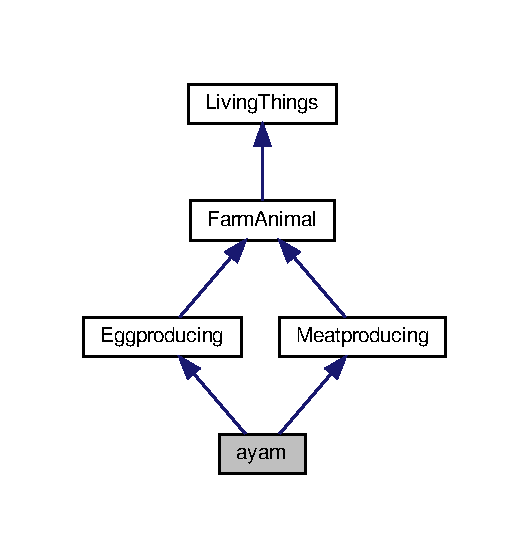
\includegraphics[width=254pt]{classayam__inherit__graph}
\end{center}
\end{figure}


Collaboration diagram for ayam\+:
\nopagebreak
\begin{figure}[H]
\begin{center}
\leavevmode
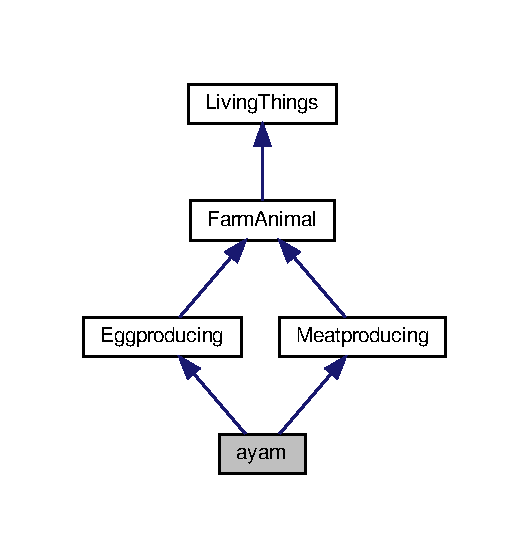
\includegraphics[width=254pt]{classayam__coll__graph}
\end{center}
\end{figure}
\subsection*{Public Member Functions}
\begin{DoxyCompactItemize}
\item 
\mbox{\Hypertarget{classayam_a1f1fdc71bbe1b0b5ff5801792c36ef03}\label{classayam_a1f1fdc71bbe1b0b5ff5801792c36ef03}} 
{\bfseries ayam} (int posX, int posY)
\item 
\mbox{\Hypertarget{classayam_a7af89a6f6a645682f4c55d4dc8a6877c}\label{classayam_a7af89a6f6a645682f4c55d4dc8a6877c}} 
\hyperlink{classayam_a7af89a6f6a645682f4c55d4dc8a6877c}{$\sim$ayam} ()
\begin{DoxyCompactList}\small\item\em constructor \end{DoxyCompactList}\item 
\mbox{\Hypertarget{classayam_a876d7b50502197028803b83a3bfe68fc}\label{classayam_a876d7b50502197028803b83a3bfe68fc}} 
void \hyperlink{classayam_a876d7b50502197028803b83a3bfe68fc}{move} ()
\begin{DoxyCompactList}\small\item\em destructor \end{DoxyCompactList}\item 
\mbox{\Hypertarget{classayam_a3f93686590f6e22c28a0d36d6db0322c}\label{classayam_a3f93686590f6e22c28a0d36d6db0322c}} 
void {\bfseries talk} ()
\item 
\mbox{\Hypertarget{classayam_a1c0d6e74ce4349de2ee7203f5328711a}\label{classayam_a1c0d6e74ce4349de2ee7203f5328711a}} 
void {\bfseries eat} ()
\item 
\mbox{\Hypertarget{classayam_a0fb6f180b3cde59dfbe9107198df6566}\label{classayam_a0fb6f180b3cde59dfbe9107198df6566}} 
string {\bfseries get\+Product} ()
\item 
\mbox{\Hypertarget{classayam_a42b927ca15fa2720766d0abfc6505b3a}\label{classayam_a42b927ca15fa2720766d0abfc6505b3a}} 
int {\bfseries getcount\+TelurA} () const
\item 
\mbox{\Hypertarget{classayam_aa9f0e9dd312dc8ed0dcba46f94a77d9a}\label{classayam_aa9f0e9dd312dc8ed0dcba46f94a77d9a}} 
int \hyperlink{classayam_aa9f0e9dd312dc8ed0dcba46f94a77d9a}{get\+Full} ()
\begin{DoxyCompactList}\small\item\em menghitung jumlah telur yang dihasilkan \end{DoxyCompactList}\item 
\mbox{\Hypertarget{classayam_aca2103a6a0565ab841f5bebc045f61c7}\label{classayam_aca2103a6a0565ab841f5bebc045f61c7}} 
void \hyperlink{classayam_aca2103a6a0565ab841f5bebc045f61c7}{set\+Full} (int Full)
\begin{DoxyCompactList}\small\item\em getter \end{DoxyCompactList}\end{DoxyCompactItemize}
\subsection*{Additional Inherited Members}


The documentation for this class was generated from the following file\+:\begin{DoxyCompactItemize}
\item 
ayam.\+h\end{DoxyCompactItemize}

\hypertarget{classbabi}{}\section{babi Class Reference}
\label{classbabi}\index{babi@{babi}}


Inheritance diagram for babi\+:
\nopagebreak
\begin{figure}[H]
\begin{center}
\leavevmode
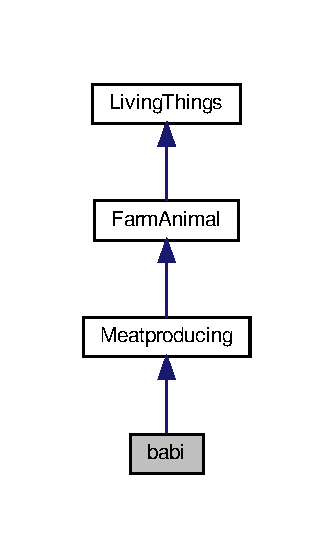
\includegraphics[width=160pt]{classbabi__inherit__graph}
\end{center}
\end{figure}


Collaboration diagram for babi\+:
\nopagebreak
\begin{figure}[H]
\begin{center}
\leavevmode
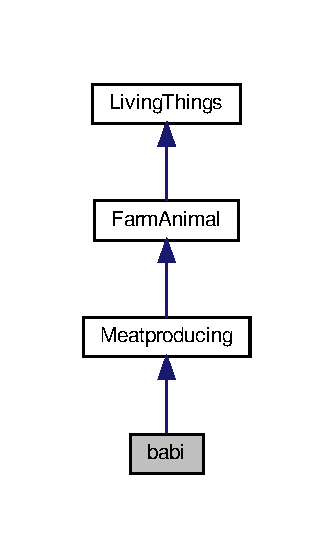
\includegraphics[width=160pt]{classbabi__coll__graph}
\end{center}
\end{figure}
\subsection*{Public Member Functions}
\begin{DoxyCompactItemize}
\item 
\mbox{\Hypertarget{classbabi_a8a0eaad29a7457b8f0a8c21c658f9a05}\label{classbabi_a8a0eaad29a7457b8f0a8c21c658f9a05}} 
{\bfseries babi} (int posX, int posY)
\item 
\mbox{\Hypertarget{classbabi_a944fb4f134cf9bf637a0855a4918d684}\label{classbabi_a944fb4f134cf9bf637a0855a4918d684}} 
void {\bfseries move} (\hyperlink{classCell}{Cell} \&\+\_\+c)
\item 
\mbox{\Hypertarget{classbabi_a2c18230abf410234e222bca1effe4d40}\label{classbabi_a2c18230abf410234e222bca1effe4d40}} 
void {\bfseries talk} ()
\item 
\mbox{\Hypertarget{classbabi_a6832fa65d6d5bd0838603c7496f6c3f1}\label{classbabi_a6832fa65d6d5bd0838603c7496f6c3f1}} 
void {\bfseries eat} (\hyperlink{classCell}{Cell} \&\+\_\+c)
\item 
\mbox{\Hypertarget{classbabi_ab439b42715b304718d2176379ba168c4}\label{classbabi_ab439b42715b304718d2176379ba168c4}} 
string {\bfseries get\+Char} ()
\item 
\mbox{\Hypertarget{classbabi_ae806759f4a9e17689c9056512173ef0e}\label{classbabi_ae806759f4a9e17689c9056512173ef0e}} 
void {\bfseries get\+Product} ()
\item 
\mbox{\Hypertarget{classbabi_af3f2e9d1b45c036f751a0f1e7aa64c32}\label{classbabi_af3f2e9d1b45c036f751a0f1e7aa64c32}} 
int {\bfseries getcount\+Pork} () const
\item 
\mbox{\Hypertarget{classbabi_a719415a9f2472843122d5f2c7e5920fa}\label{classbabi_a719415a9f2472843122d5f2c7e5920fa}} 
int {\bfseries get\+Full} ()
\item 
\mbox{\Hypertarget{classbabi_abd5372713081247b04ea16042f81d940}\label{classbabi_abd5372713081247b04ea16042f81d940}} 
void {\bfseries set\+Full} (int Full)
\item 
\mbox{\Hypertarget{classbabi_ad84b011867ac045d89c273fe155c91e4}\label{classbabi_ad84b011867ac045d89c273fe155c91e4}} 
void {\bfseries Print} ()
\end{DoxyCompactItemize}
\subsection*{Additional Inherited Members}


The documentation for this class was generated from the following files\+:\begin{DoxyCompactItemize}
\item 
babi.\+h\item 
babi.\+cpp\end{DoxyCompactItemize}

\hypertarget{classBBQ}{}\section{B\+BQ Class Reference}
\label{classBBQ}\index{B\+BQ@{B\+BQ}}


{\ttfamily \#include $<$B\+B\+Q.\+h$>$}



Inheritance diagram for B\+BQ\+:
\nopagebreak
\begin{figure}[H]
\begin{center}
\leavevmode
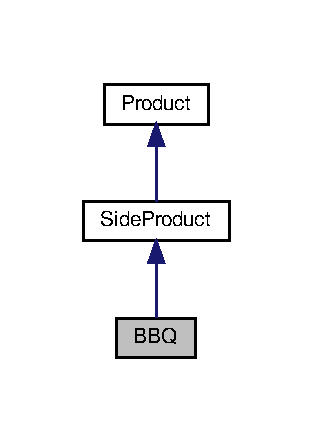
\includegraphics[width=150pt]{classBBQ__inherit__graph}
\end{center}
\end{figure}


Collaboration diagram for B\+BQ\+:
\nopagebreak
\begin{figure}[H]
\begin{center}
\leavevmode
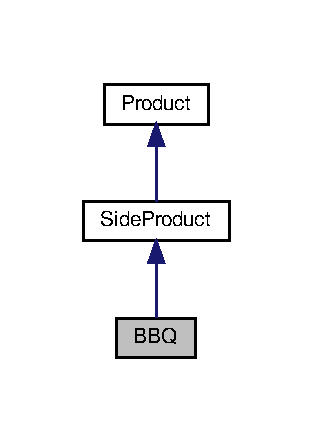
\includegraphics[width=150pt]{classBBQ__coll__graph}
\end{center}
\end{figure}
\subsection*{Public Member Functions}
\begin{DoxyCompactItemize}
\item 
\mbox{\Hypertarget{classBBQ_ae61d496afe48742d20202cc59ab8ee6f}\label{classBBQ_ae61d496afe48742d20202cc59ab8ee6f}} 
{\bfseries B\+BQ} (int portion)
\end{DoxyCompactItemize}
\subsection*{Additional Inherited Members}


\subsection{Detailed Description}
\hyperlink{classBBQ}{B\+BQ} class.

\begin{DoxyAuthor}{Author}
Ghazwan S. M. \href{mailto:ghazwan.sihamudin@gmail.com}{\tt ghazwan.\+sihamudin@gmail.\+com} 
\end{DoxyAuthor}
\begin{DoxySince}{Since}
2019.\+03.\+17 
\end{DoxySince}


The documentation for this class was generated from the following files\+:\begin{DoxyCompactItemize}
\item 
B\+B\+Q.\+h\item 
B\+B\+Q.\+cpp\end{DoxyCompactItemize}

\hypertarget{classbebek}{}\section{bebek Class Reference}
\label{classbebek}\index{bebek@{bebek}}


{\ttfamily \#include $<$bebek.\+h$>$}



Inheritance diagram for bebek\+:
\nopagebreak
\begin{figure}[H]
\begin{center}
\leavevmode
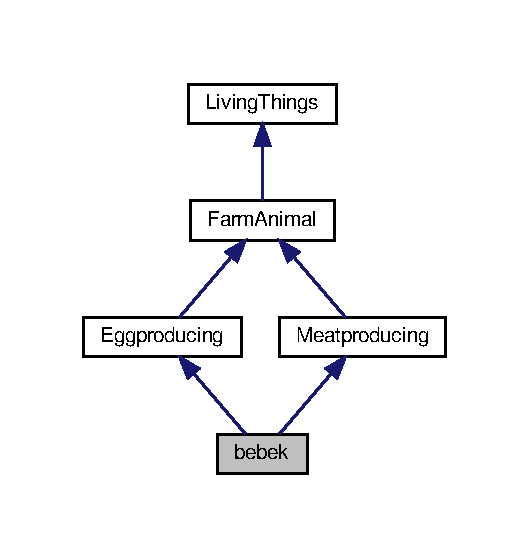
\includegraphics[width=254pt]{classbebek__inherit__graph}
\end{center}
\end{figure}


Collaboration diagram for bebek\+:
\nopagebreak
\begin{figure}[H]
\begin{center}
\leavevmode
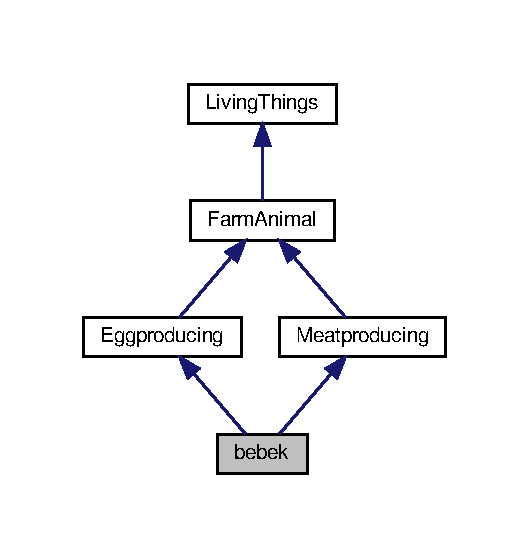
\includegraphics[width=254pt]{classbebek__coll__graph}
\end{center}
\end{figure}
\subsection*{Public Member Functions}
\begin{DoxyCompactItemize}
\item 
\mbox{\Hypertarget{classbebek_a2ee5c95e76b1895eb3ebf401f25b989e}\label{classbebek_a2ee5c95e76b1895eb3ebf401f25b989e}} 
{\bfseries bebek} (int posX, int posY)
\item 
\mbox{\Hypertarget{classbebek_afbb31871852380c811e41b1024c4ef93}\label{classbebek_afbb31871852380c811e41b1024c4ef93}} 
void {\bfseries move} (int posX, int posY)
\item 
\mbox{\Hypertarget{classbebek_a0347ebaf065829f58091d8ef0084ddf7}\label{classbebek_a0347ebaf065829f58091d8ef0084ddf7}} 
void {\bfseries talk} ()
\item 
\mbox{\Hypertarget{classbebek_ad3bafaac86ad4a25a306fdd7e787ad25}\label{classbebek_ad3bafaac86ad4a25a306fdd7e787ad25}} 
void {\bfseries eat} ()
\item 
\mbox{\Hypertarget{classbebek_a1476735835d8295a99d32058a5a839e4}\label{classbebek_a1476735835d8295a99d32058a5a839e4}} 
string {\bfseries get\+Product} ()
\item 
\mbox{\Hypertarget{classbebek_a819a9382ba77475b6226d66b3accdf17}\label{classbebek_a819a9382ba77475b6226d66b3accdf17}} 
int {\bfseries getcount\+TelurB} () const
\item 
\mbox{\Hypertarget{classbebek_ab4a19af30bd41e155db357d58c975bf2}\label{classbebek_ab4a19af30bd41e155db357d58c975bf2}} 
int {\bfseries get\+Full} ()
\item 
\mbox{\Hypertarget{classbebek_aa68ecf45df676aa449d075a82b3c748c}\label{classbebek_aa68ecf45df676aa449d075a82b3c748c}} 
void {\bfseries set\+Full} (int Full)
\end{DoxyCompactItemize}
\subsection*{Additional Inherited Members}


\subsection{Detailed Description}
bebek class. Class bebek ,turunan meat producing \begin{DoxyAuthor}{Author}
13517090 
\end{DoxyAuthor}
\begin{DoxySince}{Since}
2019.\+03.\+17 
\end{DoxySince}


The documentation for this class was generated from the following file\+:\begin{DoxyCompactItemize}
\item 
bebek.\+h\end{DoxyCompactItemize}

\hypertarget{classCell}{}\section{Cell Class Reference}
\label{classCell}\index{Cell@{Cell}}


Inheritance diagram for Cell\+:
\nopagebreak
\begin{figure}[H]
\begin{center}
\leavevmode
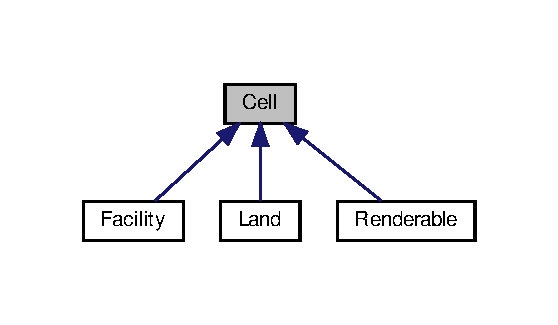
\includegraphics[width=128pt]{classCell__inherit__graph}
\end{center}
\end{figure}
\subsection*{Public Member Functions}
\begin{DoxyCompactItemize}
\item 
\mbox{\Hypertarget{classCell_a00ad90ebf8a8397e7e6686a0c53a129c}\label{classCell_a00ad90ebf8a8397e7e6686a0c53a129c}} 
void {\bfseries set\+Sizex} (int \+\_\+x)
\item 
\mbox{\Hypertarget{classCell_ae0dbdae2b884f76adcfd445ef3cbb26f}\label{classCell_ae0dbdae2b884f76adcfd445ef3cbb26f}} 
void {\bfseries set\+Sizey} (int \+\_\+y)
\item 
\mbox{\Hypertarget{classCell_a4fb0c2cf923dda5f0c99374ae83bc5df}\label{classCell_a4fb0c2cf923dda5f0c99374ae83bc5df}} 
int {\bfseries get\+Sizex} ()
\item 
\mbox{\Hypertarget{classCell_abe016b4186be0a92f5ad0d28f6742a1d}\label{classCell_abe016b4186be0a92f5ad0d28f6742a1d}} 
int {\bfseries get\+Sizey} ()
\item 
\mbox{\Hypertarget{classCell_a4856fe7f442321d862e21153cc8952e3}\label{classCell_a4856fe7f442321d862e21153cc8952e3}} 
int {\bfseries get\+Element} (int x, int y)
\item 
\mbox{\Hypertarget{classCell_aeaa88a5d7cde0de11ffee7788d3412bd}\label{classCell_aeaa88a5d7cde0de11ffee7788d3412bd}} 
string {\bfseries get\+Properties} (int value)
\item 
\mbox{\Hypertarget{classCell_a48bc12937e6590e6434dd81eedc55986}\label{classCell_a48bc12937e6590e6434dd81eedc55986}} 
bool {\bfseries is\+Empty\+Cell} (int x, int y)
\end{DoxyCompactItemize}


The documentation for this class was generated from the following file\+:\begin{DoxyCompactItemize}
\item 
Cell.\+h\end{DoxyCompactItemize}

\hypertarget{classChickenEgg}{}\section{Chicken\+Egg Class Reference}
\label{classChickenEgg}\index{Chicken\+Egg@{Chicken\+Egg}}


{\ttfamily \#include $<$Chicken\+Egg.\+h$>$}



Inheritance diagram for Chicken\+Egg\+:
\nopagebreak
\begin{figure}[H]
\begin{center}
\leavevmode
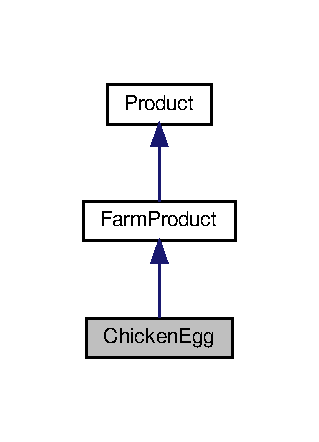
\includegraphics[width=153pt]{classChickenEgg__inherit__graph}
\end{center}
\end{figure}


Collaboration diagram for Chicken\+Egg\+:
\nopagebreak
\begin{figure}[H]
\begin{center}
\leavevmode
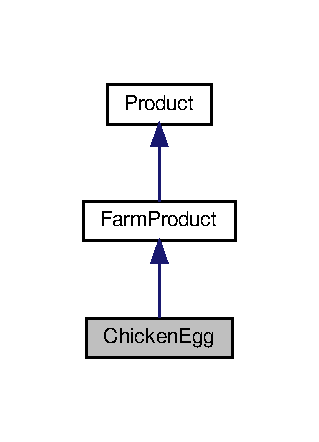
\includegraphics[width=153pt]{classChickenEgg__coll__graph}
\end{center}
\end{figure}
\subsection*{Additional Inherited Members}


\subsection{Detailed Description}
\hyperlink{classChickenEgg}{Chicken\+Egg} class.

\begin{DoxyAuthor}{Author}
Ghazwan S. M. \href{mailto:ghazwan.sihamudin@gmail.com}{\tt ghazwan.\+sihamudin@gmail.\+com} 
\end{DoxyAuthor}
\begin{DoxySince}{Since}
2019.\+03.\+17 
\end{DoxySince}


The documentation for this class was generated from the following file\+:\begin{DoxyCompactItemize}
\item 
Chicken\+Egg.\+h\end{DoxyCompactItemize}

\hypertarget{classChickenMeat}{}\section{Chicken\+Meat Class Reference}
\label{classChickenMeat}\index{Chicken\+Meat@{Chicken\+Meat}}


{\ttfamily \#include $<$Chicken\+Meat.\+h$>$}



Inheritance diagram for Chicken\+Meat\+:
\nopagebreak
\begin{figure}[H]
\begin{center}
\leavevmode
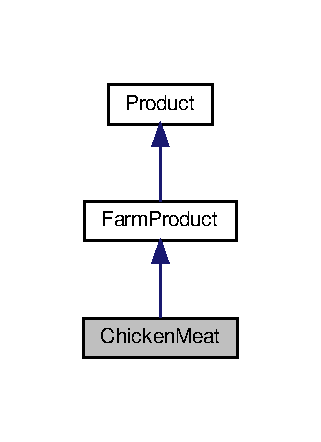
\includegraphics[width=154pt]{classChickenMeat__inherit__graph}
\end{center}
\end{figure}


Collaboration diagram for Chicken\+Meat\+:
\nopagebreak
\begin{figure}[H]
\begin{center}
\leavevmode
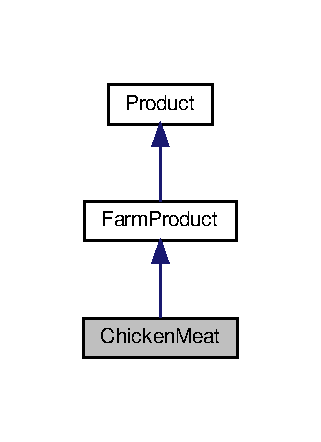
\includegraphics[width=154pt]{classChickenMeat__coll__graph}
\end{center}
\end{figure}
\subsection*{Additional Inherited Members}


\subsection{Detailed Description}
\hyperlink{classChickenMeat}{Chicken\+Meat} class.

\begin{DoxyAuthor}{Author}
Ghazwan S. M. \href{mailto:ghazwan.sihamudin@gmail.com}{\tt ghazwan.\+sihamudin@gmail.\+com} 
\end{DoxyAuthor}
\begin{DoxySince}{Since}
2019.\+03.\+17 
\end{DoxySince}


The documentation for this class was generated from the following files\+:\begin{DoxyCompactItemize}
\item 
Chicken\+Meat.\+h\item 
Chicken\+Meat.\+cpp\end{DoxyCompactItemize}

\hypertarget{classCowMeat}{}\section{Cow\+Meat Class Reference}
\label{classCowMeat}\index{Cow\+Meat@{Cow\+Meat}}


{\ttfamily \#include $<$Cow\+Meat.\+h$>$}



Inheritance diagram for Cow\+Meat\+:
\nopagebreak
\begin{figure}[H]
\begin{center}
\leavevmode
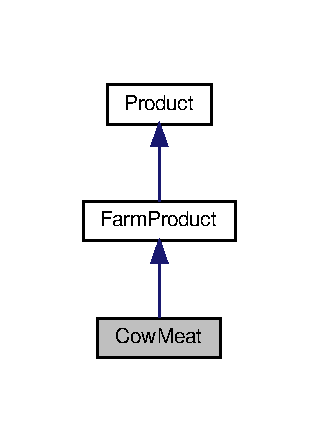
\includegraphics[width=153pt]{classCowMeat__inherit__graph}
\end{center}
\end{figure}


Collaboration diagram for Cow\+Meat\+:
\nopagebreak
\begin{figure}[H]
\begin{center}
\leavevmode
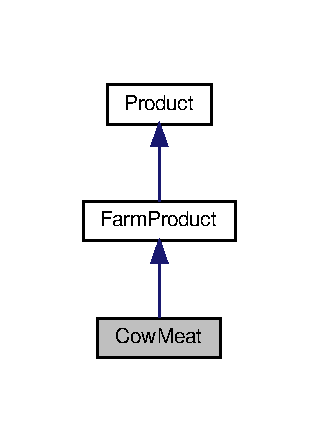
\includegraphics[width=153pt]{classCowMeat__coll__graph}
\end{center}
\end{figure}
\subsection*{Additional Inherited Members}


\subsection{Detailed Description}
\hyperlink{classCowMeat}{Cow\+Meat} class.

\begin{DoxyAuthor}{Author}
Ghazwan S. M. \href{mailto:ghazwan.sihamudin@gmail.com}{\tt ghazwan.\+sihamudin@gmail.\+com} 
\end{DoxyAuthor}
\begin{DoxySince}{Since}
2019.\+03.\+17 
\end{DoxySince}


The documentation for this class was generated from the following files\+:\begin{DoxyCompactItemize}
\item 
Cow\+Meat.\+h\item 
Cow\+Meat.\+cpp\end{DoxyCompactItemize}

\hypertarget{classCowMilk}{}\section{Cow\+Milk Class Reference}
\label{classCowMilk}\index{Cow\+Milk@{Cow\+Milk}}


{\ttfamily \#include $<$Cow\+Milk.\+h$>$}



Inheritance diagram for Cow\+Milk\+:
\nopagebreak
\begin{figure}[H]
\begin{center}
\leavevmode
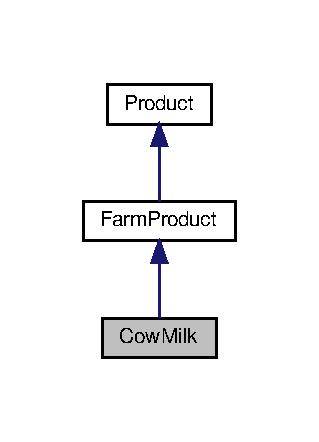
\includegraphics[width=153pt]{classCowMilk__inherit__graph}
\end{center}
\end{figure}


Collaboration diagram for Cow\+Milk\+:
\nopagebreak
\begin{figure}[H]
\begin{center}
\leavevmode
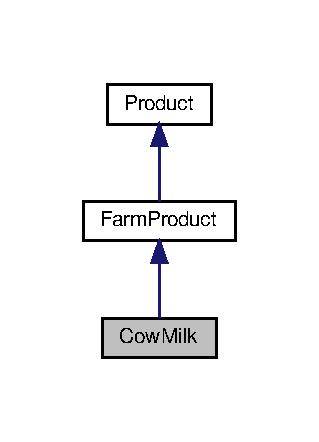
\includegraphics[width=153pt]{classCowMilk__coll__graph}
\end{center}
\end{figure}
\subsection*{Additional Inherited Members}


\subsection{Detailed Description}
\hyperlink{classCowMilk}{Cow\+Milk} class.

\begin{DoxyAuthor}{Author}
Ghazwan S. M. \href{mailto:ghazwan.sihamudin@gmail.com}{\tt ghazwan.\+sihamudin@gmail.\+com} 
\end{DoxyAuthor}
\begin{DoxySince}{Since}
2019.\+03.\+17 
\end{DoxySince}


The documentation for this class was generated from the following files\+:\begin{DoxyCompactItemize}
\item 
Cow\+Milk.\+h\item 
Cow\+Milk.\+cpp\end{DoxyCompactItemize}

\hypertarget{classdomba}{}\section{domba Class Reference}
\label{classdomba}\index{domba@{domba}}


Inheritance diagram for domba\+:
\nopagebreak
\begin{figure}[H]
\begin{center}
\leavevmode
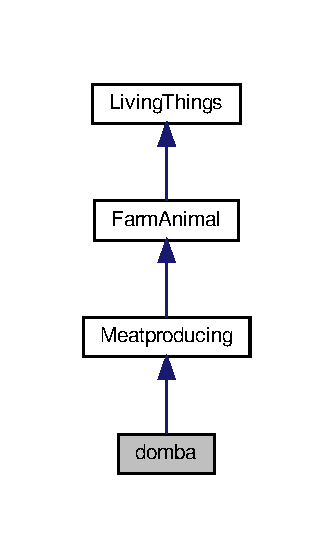
\includegraphics[width=160pt]{classdomba__inherit__graph}
\end{center}
\end{figure}


Collaboration diagram for domba\+:
\nopagebreak
\begin{figure}[H]
\begin{center}
\leavevmode
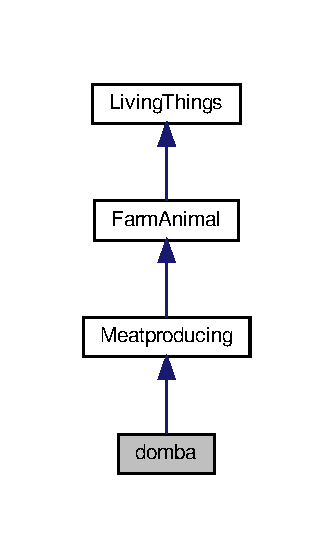
\includegraphics[width=160pt]{classdomba__coll__graph}
\end{center}
\end{figure}
\subsection*{Public Member Functions}
\begin{DoxyCompactItemize}
\item 
\mbox{\Hypertarget{classdomba_a2b68f77b04b105d52ce1c3466d13c42a}\label{classdomba_a2b68f77b04b105d52ce1c3466d13c42a}} 
{\bfseries domba} (int posX, int posY)
\item 
\mbox{\Hypertarget{classdomba_ab3afd792e6e1dc41d849ad891cf299e3}\label{classdomba_ab3afd792e6e1dc41d849ad891cf299e3}} 
void {\bfseries move} (\hyperlink{classCell}{Cell} \&\+\_\+c)
\item 
\mbox{\Hypertarget{classdomba_afbed61a200b204818b134c8c76412d55}\label{classdomba_afbed61a200b204818b134c8c76412d55}} 
void {\bfseries talk} ()
\item 
\mbox{\Hypertarget{classdomba_abc21d7405a38f4cd880de8a4f6d7b0e5}\label{classdomba_abc21d7405a38f4cd880de8a4f6d7b0e5}} 
void {\bfseries eat} (\hyperlink{classCell}{Cell} \&\+\_\+c)
\item 
\mbox{\Hypertarget{classdomba_ad2cbf646472c3aa5fecd51e0d00d1b3c}\label{classdomba_ad2cbf646472c3aa5fecd51e0d00d1b3c}} 
string {\bfseries get\+Char} ()
\item 
\mbox{\Hypertarget{classdomba_af1f02315df4888e95ac53fb29332e226}\label{classdomba_af1f02315df4888e95ac53fb29332e226}} 
void {\bfseries get\+Product} ()
\item 
\mbox{\Hypertarget{classdomba_a60ca47d7f6bc14a539d8530d0cd318be}\label{classdomba_a60ca47d7f6bc14a539d8530d0cd318be}} 
int {\bfseries get\+Count\+Lamb\+Meat} () const
\item 
\mbox{\Hypertarget{classdomba_aa54efee014f7803128d384b0b19672a6}\label{classdomba_aa54efee014f7803128d384b0b19672a6}} 
int {\bfseries get\+Full} ()
\item 
\mbox{\Hypertarget{classdomba_a89fb54203e1c9bfb9859344d2903eecf}\label{classdomba_a89fb54203e1c9bfb9859344d2903eecf}} 
void {\bfseries set\+Full} (int Full)
\item 
\mbox{\Hypertarget{classdomba_a2d48bac78090b5b9f059d464ed3b974e}\label{classdomba_a2d48bac78090b5b9f059d464ed3b974e}} 
void {\bfseries Print} ()
\end{DoxyCompactItemize}
\subsection*{Additional Inherited Members}


The documentation for this class was generated from the following files\+:\begin{DoxyCompactItemize}
\item 
domba.\+h\item 
domba.\+cpp\end{DoxyCompactItemize}

\hypertarget{classDuckEgg}{}\section{Duck\+Egg Class Reference}
\label{classDuckEgg}\index{Duck\+Egg@{Duck\+Egg}}


{\ttfamily \#include $<$Duck\+Egg.\+h$>$}



Inheritance diagram for Duck\+Egg\+:
\nopagebreak
\begin{figure}[H]
\begin{center}
\leavevmode
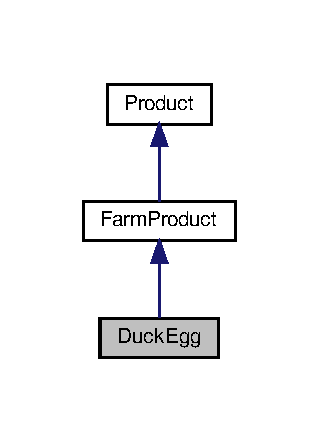
\includegraphics[width=153pt]{classDuckEgg__inherit__graph}
\end{center}
\end{figure}


Collaboration diagram for Duck\+Egg\+:
\nopagebreak
\begin{figure}[H]
\begin{center}
\leavevmode
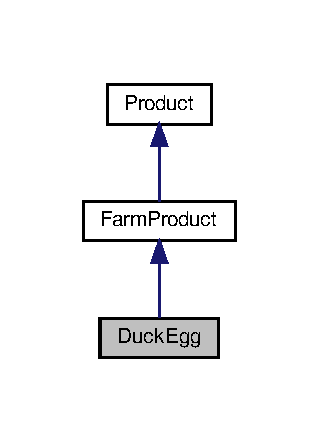
\includegraphics[width=153pt]{classDuckEgg__coll__graph}
\end{center}
\end{figure}
\subsection*{Additional Inherited Members}


\subsection{Detailed Description}
\hyperlink{classDuckEgg}{Duck\+Egg} class.

\begin{DoxyAuthor}{Author}
Ghazwan S. M. \href{mailto:ghazwan.sihamudin@gmail.com}{\tt ghazwan.\+sihamudin@gmail.\+com} 
\end{DoxyAuthor}
\begin{DoxySince}{Since}
2019.\+03.\+17 
\end{DoxySince}


The documentation for this class was generated from the following files\+:\begin{DoxyCompactItemize}
\item 
Duck\+Egg.\+h\item 
Duck\+Egg.\+cpp\end{DoxyCompactItemize}

\hypertarget{classDuckMeat}{}\section{Duck\+Meat Class Reference}
\label{classDuckMeat}\index{Duck\+Meat@{Duck\+Meat}}


{\ttfamily \#include $<$Duck\+Meat.\+h$>$}



Inheritance diagram for Duck\+Meat\+:
\nopagebreak
\begin{figure}[H]
\begin{center}
\leavevmode
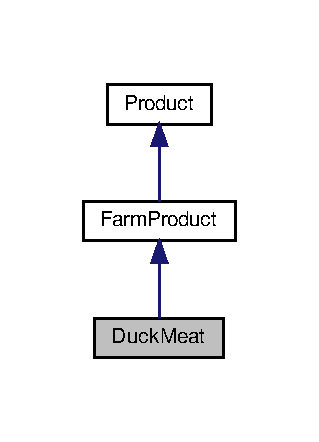
\includegraphics[width=153pt]{classDuckMeat__inherit__graph}
\end{center}
\end{figure}


Collaboration diagram for Duck\+Meat\+:
\nopagebreak
\begin{figure}[H]
\begin{center}
\leavevmode
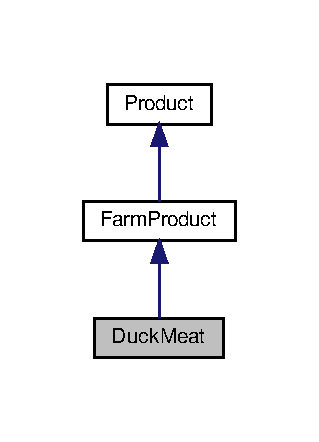
\includegraphics[width=153pt]{classDuckMeat__coll__graph}
\end{center}
\end{figure}
\subsection*{Additional Inherited Members}


\subsection{Detailed Description}
\hyperlink{classDuckMeat}{Duck\+Meat} class.

\begin{DoxyAuthor}{Author}
Ghazwan S. M. \href{mailto:ghazwan.sihamudin@gmail.com}{\tt ghazwan.\+sihamudin@gmail.\+com} 
\end{DoxyAuthor}
\begin{DoxySince}{Since}
2019.\+03.\+17 
\end{DoxySince}


The documentation for this class was generated from the following files\+:\begin{DoxyCompactItemize}
\item 
Duck\+Meat.\+h\item 
Duck\+Meat.\+cpp\end{DoxyCompactItemize}

\hypertarget{classEggproducing}{}\section{Eggproducing Class Reference}
\label{classEggproducing}\index{Eggproducing@{Eggproducing}}


{\ttfamily \#include $<$Eggproducing.\+h$>$}



Inheritance diagram for Eggproducing\+:
\nopagebreak
\begin{figure}[H]
\begin{center}
\leavevmode
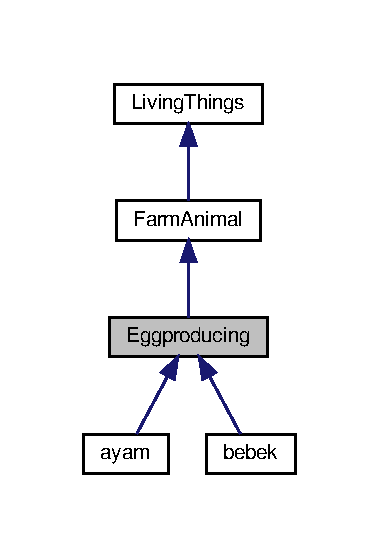
\includegraphics[width=182pt]{classEggproducing__inherit__graph}
\end{center}
\end{figure}


Collaboration diagram for Eggproducing\+:
\nopagebreak
\begin{figure}[H]
\begin{center}
\leavevmode
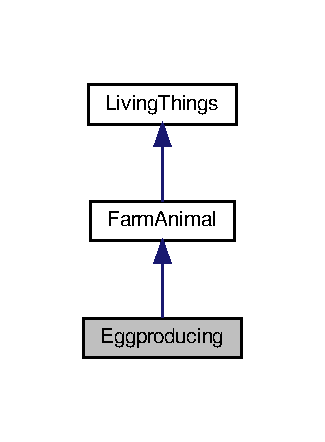
\includegraphics[width=156pt]{classEggproducing__coll__graph}
\end{center}
\end{figure}
\subsection*{Public Member Functions}
\begin{DoxyCompactItemize}
\item 
\mbox{\Hypertarget{classEggproducing_a61b4dcb66766bd42d50b965c7e1e4b82}\label{classEggproducing_a61b4dcb66766bd42d50b965c7e1e4b82}} 
{\bfseries Eggproducing} (int x, int y)
\end{DoxyCompactItemize}
\subsection*{Static Public Member Functions}
\begin{DoxyCompactItemize}
\item 
\mbox{\Hypertarget{classEggproducing_abab358d9eec12cca84e962f4e665afb8}\label{classEggproducing_abab358d9eec12cca84e962f4e665afb8}} 
static int {\bfseries getjlh\+EggP} ()
\end{DoxyCompactItemize}
\subsection*{Additional Inherited Members}


\subsection{Detailed Description}
\hyperlink{classEggproducing}{Eggproducing} class Class hewan penghasil telur ,kelas turunan dari farm animal \begin{DoxyAuthor}{Author}
13517090 
\end{DoxyAuthor}
\begin{DoxySince}{Since}
2019.\+03.\+17 
\end{DoxySince}


The documentation for this class was generated from the following file\+:\begin{DoxyCompactItemize}
\item 
Eggproducing.\+h\end{DoxyCompactItemize}

\hypertarget{classFacility}{}\section{Facility Class Reference}
\label{classFacility}\index{Facility@{Facility}}


Inheritance diagram for Facility\+:
\nopagebreak
\begin{figure}[H]
\begin{center}
\leavevmode
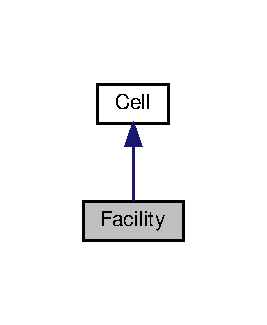
\includegraphics[width=128pt]{classFacility__inherit__graph}
\end{center}
\end{figure}


Collaboration diagram for Facility\+:
\nopagebreak
\begin{figure}[H]
\begin{center}
\leavevmode
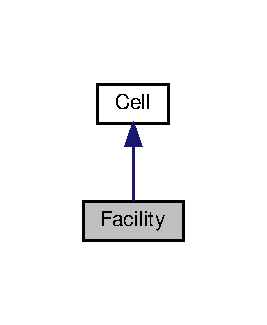
\includegraphics[width=128pt]{classFacility__coll__graph}
\end{center}
\end{figure}
\subsection*{Public Member Functions}
\begin{DoxyCompactItemize}
\item 
\mbox{\Hypertarget{classFacility_a7c78504d3a00acecd711a8b1660bdd75}\label{classFacility_a7c78504d3a00acecd711a8b1660bdd75}} 
int {\bfseries get\+WellX} ()
\item 
\mbox{\Hypertarget{classFacility_a2a05eb6d177de7c03ed1a49dc3dd0a23}\label{classFacility_a2a05eb6d177de7c03ed1a49dc3dd0a23}} 
int {\bfseries get\+WellY} ()
\item 
\mbox{\Hypertarget{classFacility_a9da908938a996df43fa0933469a4a60f}\label{classFacility_a9da908938a996df43fa0933469a4a60f}} 
int {\bfseries get\+MixerX} ()
\item 
\mbox{\Hypertarget{classFacility_a83974275a93f061cc7b5c080de5f2c8e}\label{classFacility_a83974275a93f061cc7b5c080de5f2c8e}} 
int {\bfseries get\+MixerY} ()
\item 
\mbox{\Hypertarget{classFacility_a800ac7290dbba8f15c8b0d9446073de0}\label{classFacility_a800ac7290dbba8f15c8b0d9446073de0}} 
int {\bfseries get\+TruckX} ()
\item 
\mbox{\Hypertarget{classFacility_aed8bda7a1dfc76391903bcf92b35ab13}\label{classFacility_aed8bda7a1dfc76391903bcf92b35ab13}} 
int {\bfseries get\+TruckY} ()
\end{DoxyCompactItemize}


The documentation for this class was generated from the following files\+:\begin{DoxyCompactItemize}
\item 
Facility.\+h\item 
Facility.\+cpp\end{DoxyCompactItemize}

\hypertarget{classFarmAnimal}{}\section{Farm\+Animal Class Reference}
\label{classFarmAnimal}\index{Farm\+Animal@{Farm\+Animal}}


Inheritance diagram for Farm\+Animal\+:
\nopagebreak
\begin{figure}[H]
\begin{center}
\leavevmode
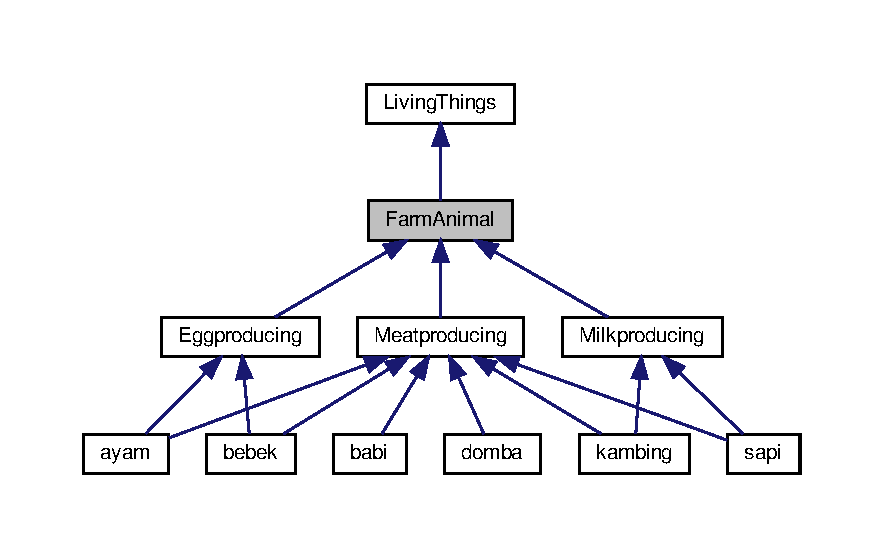
\includegraphics[width=350pt]{classFarmAnimal__inherit__graph}
\end{center}
\end{figure}


Collaboration diagram for Farm\+Animal\+:
\nopagebreak
\begin{figure}[H]
\begin{center}
\leavevmode
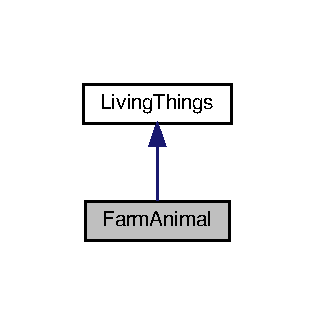
\includegraphics[width=151pt]{classFarmAnimal__coll__graph}
\end{center}
\end{figure}
\subsection*{Public Member Functions}
\begin{DoxyCompactItemize}
\item 
\mbox{\Hypertarget{classFarmAnimal_adea13b232d5f3967a473e2e062d33ee8}\label{classFarmAnimal_adea13b232d5f3967a473e2e062d33ee8}} 
{\bfseries Farm\+Animal} (int x, int y)
\item 
\mbox{\Hypertarget{classFarmAnimal_ab47da74e7a3644058d69b70b19508022}\label{classFarmAnimal_ab47da74e7a3644058d69b70b19508022}} 
virtual void {\bfseries eat} (\hyperlink{classCell}{Cell} \&\+\_\+c)=0
\item 
\mbox{\Hypertarget{classFarmAnimal_ad636494e597db9fc13ffddd3a405bfeb}\label{classFarmAnimal_ad636494e597db9fc13ffddd3a405bfeb}} 
virtual string {\bfseries get\+Char} ()=0
\item 
\mbox{\Hypertarget{classFarmAnimal_ad236b0044f0feb479fafd90fde03f3c1}\label{classFarmAnimal_ad236b0044f0feb479fafd90fde03f3c1}} 
virtual void {\bfseries get\+Product} ()=0
\item 
\mbox{\Hypertarget{classFarmAnimal_a6e60fd2db37d4c521d9905310754ab85}\label{classFarmAnimal_a6e60fd2db37d4c521d9905310754ab85}} 
virtual void {\bfseries Print} ()=0
\item 
\mbox{\Hypertarget{classFarmAnimal_a3a741d8636f20916bef977111e8e1657}\label{classFarmAnimal_a3a741d8636f20916bef977111e8e1657}} 
virtual void {\bfseries set\+Full} (int Full)=0
\item 
\mbox{\Hypertarget{classFarmAnimal_ab083c4b544344e912e7c8cb372e3461e}\label{classFarmAnimal_ab083c4b544344e912e7c8cb372e3461e}} 
virtual void {\bfseries move} (\hyperlink{classCell}{Cell} \&\+\_\+c)=0
\item 
\mbox{\Hypertarget{classFarmAnimal_ae554d658eaa9f4f6fc3971f8ab87c78a}\label{classFarmAnimal_ae554d658eaa9f4f6fc3971f8ab87c78a}} 
int {\bfseries get\+PosX} ()
\item 
\mbox{\Hypertarget{classFarmAnimal_acbf8b1288f4ccb80610e87f7072e6838}\label{classFarmAnimal_acbf8b1288f4ccb80610e87f7072e6838}} 
int {\bfseries get\+PosY} ()
\item 
\mbox{\Hypertarget{classFarmAnimal_ada8a7127ac5ec7baec9277262b95178e}\label{classFarmAnimal_ada8a7127ac5ec7baec9277262b95178e}} 
void {\bfseries set\+PosX} (int x)
\item 
\mbox{\Hypertarget{classFarmAnimal_a327c4fc53e4dc3a470a7cfb49942dfa5}\label{classFarmAnimal_a327c4fc53e4dc3a470a7cfb49942dfa5}} 
void {\bfseries set\+PosY} (int y)
\item 
\mbox{\Hypertarget{classFarmAnimal_a6ab91d1c11fb077e4938f6c81ec5adaf}\label{classFarmAnimal_a6ab91d1c11fb077e4938f6c81ec5adaf}} 
bool {\bfseries get\+Status} ()
\item 
\mbox{\Hypertarget{classFarmAnimal_a7166b5b2970eaf4c8e4376fa0b230c08}\label{classFarmAnimal_a7166b5b2970eaf4c8e4376fa0b230c08}} 
void {\bfseries set\+Status} (bool cek)
\end{DoxyCompactItemize}
\subsection*{Static Public Member Functions}
\begin{DoxyCompactItemize}
\item 
\mbox{\Hypertarget{classFarmAnimal_a8430146a93c89ce6f674286a7ccfca18}\label{classFarmAnimal_a8430146a93c89ce6f674286a7ccfca18}} 
static int {\bfseries get\+Count\+Animal} ()
\end{DoxyCompactItemize}
\subsection*{Protected Attributes}
\begin{DoxyCompactItemize}
\item 
\mbox{\Hypertarget{classFarmAnimal_a05002cb10f4fcc02f6723a6a118e65b4}\label{classFarmAnimal_a05002cb10f4fcc02f6723a6a118e65b4}} 
int {\bfseries Full}
\item 
\mbox{\Hypertarget{classFarmAnimal_a35a7ed9424ab665d03045c3c0bbdfca7}\label{classFarmAnimal_a35a7ed9424ab665d03045c3c0bbdfca7}} 
bool {\bfseries status}
\end{DoxyCompactItemize}


The documentation for this class was generated from the following files\+:\begin{DoxyCompactItemize}
\item 
Farm\+Animal.\+h\item 
Farm\+Animal.\+cpp\end{DoxyCompactItemize}

\hypertarget{classFarmProduct}{}\section{Farm\+Product Class Reference}
\label{classFarmProduct}\index{Farm\+Product@{Farm\+Product}}


{\ttfamily \#include $<$Farm\+Product.\+h$>$}



Inheritance diagram for Farm\+Product\+:
\nopagebreak
\begin{figure}[H]
\begin{center}
\leavevmode
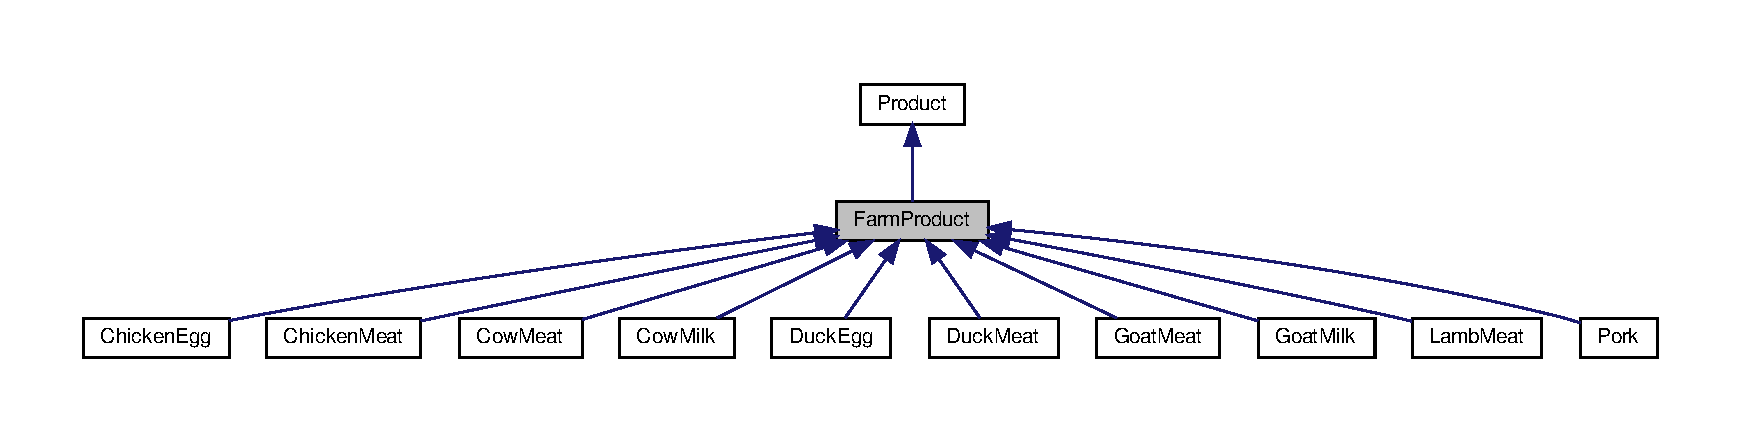
\includegraphics[width=350pt]{classFarmProduct__inherit__graph}
\end{center}
\end{figure}


Collaboration diagram for Farm\+Product\+:
\nopagebreak
\begin{figure}[H]
\begin{center}
\leavevmode
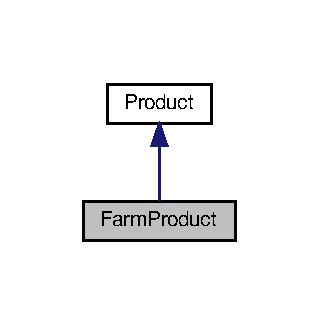
\includegraphics[width=153pt]{classFarmProduct__coll__graph}
\end{center}
\end{figure}
\subsection*{Public Member Functions}
\begin{DoxyCompactItemize}
\item 
int \hyperlink{classFarmProduct_ae169937bd043517efa0a05be844aaa35}{get\+Product\+Value} ()
\item 
int \hyperlink{classFarmProduct_a2a7526789b3ab01a8fda7773aa2c0565}{get\+Expire\+Value} ()
\item 
void \hyperlink{classFarmProduct_aea484f8f23984c14e0014fa7c35b9629}{set\+Expire\+Value} ()
\item 
bool \hyperlink{classFarmProduct_a18cb875372c4e24ef79615bcd47a110e}{is\+Expire} ()
\end{DoxyCompactItemize}
\subsection*{Additional Inherited Members}


\subsection{Detailed Description}
\hyperlink{classFarmProduct}{Farm\+Product} class.

\begin{DoxyAuthor}{Author}
Ghazwan S. M. \href{mailto:ghazwan.sihamudin@gmail.com}{\tt ghazwan.\+sihamudin@gmail.\+com} 
\end{DoxyAuthor}
\begin{DoxySince}{Since}
2019.\+03.\+17 
\end{DoxySince}


\subsection{Member Function Documentation}
\mbox{\Hypertarget{classFarmProduct_a2a7526789b3ab01a8fda7773aa2c0565}\label{classFarmProduct_a2a7526789b3ab01a8fda7773aa2c0565}} 
\index{Farm\+Product@{Farm\+Product}!get\+Expire\+Value@{get\+Expire\+Value}}
\index{get\+Expire\+Value@{get\+Expire\+Value}!Farm\+Product@{Farm\+Product}}
\subsubsection{\texorpdfstring{get\+Expire\+Value()}{getExpireValue()}}
{\footnotesize\ttfamily int Farm\+Product\+::get\+Expire\+Value (\begin{DoxyParamCaption}{ }\end{DoxyParamCaption})\hspace{0.3cm}{\ttfamily [virtual]}}

Get the expire value of the product. \begin{DoxyReturn}{Returns}
int expire value. 
\end{DoxyReturn}


Implements \hyperlink{classProduct_a739031c520fb9e376da3d3fc2955c7e7}{Product}.

\mbox{\Hypertarget{classFarmProduct_ae169937bd043517efa0a05be844aaa35}\label{classFarmProduct_ae169937bd043517efa0a05be844aaa35}} 
\index{Farm\+Product@{Farm\+Product}!get\+Product\+Value@{get\+Product\+Value}}
\index{get\+Product\+Value@{get\+Product\+Value}!Farm\+Product@{Farm\+Product}}
\subsubsection{\texorpdfstring{get\+Product\+Value()}{getProductValue()}}
{\footnotesize\ttfamily int Farm\+Product\+::get\+Product\+Value (\begin{DoxyParamCaption}{ }\end{DoxyParamCaption})\hspace{0.3cm}{\ttfamily [virtual]}}

Get the product value. \begin{DoxyReturn}{Returns}
int product value. 
\end{DoxyReturn}


Implements \hyperlink{classProduct_a5c56d625cae28f43b626578ac4611e43}{Product}.

\mbox{\Hypertarget{classFarmProduct_a18cb875372c4e24ef79615bcd47a110e}\label{classFarmProduct_a18cb875372c4e24ef79615bcd47a110e}} 
\index{Farm\+Product@{Farm\+Product}!is\+Expire@{is\+Expire}}
\index{is\+Expire@{is\+Expire}!Farm\+Product@{Farm\+Product}}
\subsubsection{\texorpdfstring{is\+Expire()}{isExpire()}}
{\footnotesize\ttfamily bool Farm\+Product\+::is\+Expire (\begin{DoxyParamCaption}{ }\end{DoxyParamCaption})\hspace{0.3cm}{\ttfamily [virtual]}}

Get the product expire condition. \begin{DoxyReturn}{Returns}
bool expire condition. 
\end{DoxyReturn}


Implements \hyperlink{classProduct_aec86d25d77417014f8780ea65416bac7}{Product}.

\mbox{\Hypertarget{classFarmProduct_aea484f8f23984c14e0014fa7c35b9629}\label{classFarmProduct_aea484f8f23984c14e0014fa7c35b9629}} 
\index{Farm\+Product@{Farm\+Product}!set\+Expire\+Value@{set\+Expire\+Value}}
\index{set\+Expire\+Value@{set\+Expire\+Value}!Farm\+Product@{Farm\+Product}}
\subsubsection{\texorpdfstring{set\+Expire\+Value()}{setExpireValue()}}
{\footnotesize\ttfamily void Farm\+Product\+::set\+Expire\+Value (\begin{DoxyParamCaption}{ }\end{DoxyParamCaption})\hspace{0.3cm}{\ttfamily [virtual]}}

Reduce the expire value of the product by 1. 

Implements \hyperlink{classProduct_a84aba139efc9cbcb05d47de168645463}{Product}.



The documentation for this class was generated from the following files\+:\begin{DoxyCompactItemize}
\item 
Farm\+Product.\+h\item 
Farm\+Product.\+cpp\end{DoxyCompactItemize}

\hypertarget{classGoatMeat}{}\section{Goat\+Meat Class Reference}
\label{classGoatMeat}\index{Goat\+Meat@{Goat\+Meat}}


{\ttfamily \#include $<$Goat\+Meat.\+h$>$}



Inheritance diagram for Goat\+Meat\+:
\nopagebreak
\begin{figure}[H]
\begin{center}
\leavevmode
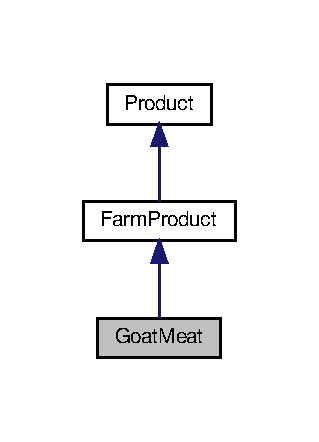
\includegraphics[width=153pt]{classGoatMeat__inherit__graph}
\end{center}
\end{figure}


Collaboration diagram for Goat\+Meat\+:
\nopagebreak
\begin{figure}[H]
\begin{center}
\leavevmode
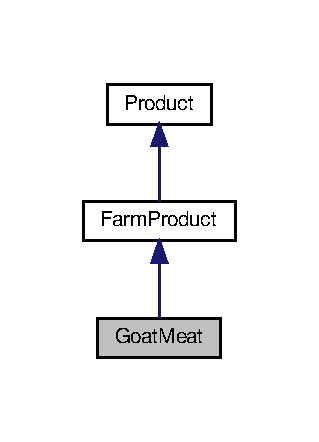
\includegraphics[width=153pt]{classGoatMeat__coll__graph}
\end{center}
\end{figure}
\subsection*{Additional Inherited Members}


\subsection{Detailed Description}
\hyperlink{classGoatMeat}{Goat\+Meat} class.

\begin{DoxyAuthor}{Author}
Ghazwan S. M. \href{mailto:ghazwan.sihamudin@gmail.com}{\tt ghazwan.\+sihamudin@gmail.\+com} 
\end{DoxyAuthor}
\begin{DoxySince}{Since}
2019.\+03.\+17 
\end{DoxySince}


The documentation for this class was generated from the following files\+:\begin{DoxyCompactItemize}
\item 
Goat\+Meat.\+h\item 
Lamb\+Meat.\+h\end{DoxyCompactItemize}

\hypertarget{classGoatMilk}{}\section{Goat\+Milk Class Reference}
\label{classGoatMilk}\index{Goat\+Milk@{Goat\+Milk}}


{\ttfamily \#include $<$Goat\+Milk.\+h$>$}



Inheritance diagram for Goat\+Milk\+:
\nopagebreak
\begin{figure}[H]
\begin{center}
\leavevmode
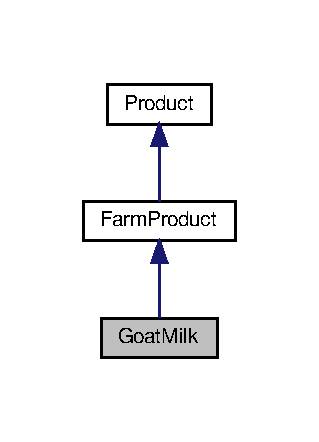
\includegraphics[width=153pt]{classGoatMilk__inherit__graph}
\end{center}
\end{figure}


Collaboration diagram for Goat\+Milk\+:
\nopagebreak
\begin{figure}[H]
\begin{center}
\leavevmode
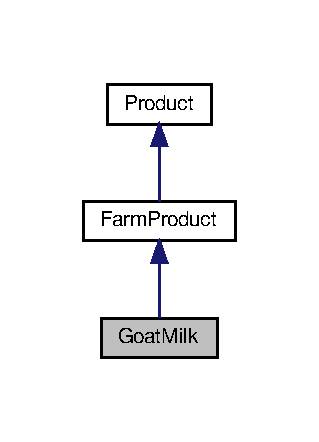
\includegraphics[width=153pt]{classGoatMilk__coll__graph}
\end{center}
\end{figure}
\subsection*{Additional Inherited Members}


\subsection{Detailed Description}
\hyperlink{classGoatMilk}{Goat\+Milk} class.

\begin{DoxyAuthor}{Author}
Ghazwan S. M. \href{mailto:ghazwan.sihamudin@gmail.com}{\tt ghazwan.\+sihamudin@gmail.\+com} 
\end{DoxyAuthor}
\begin{DoxySince}{Since}
2019.\+03.\+17 
\end{DoxySince}


The documentation for this class was generated from the following file\+:\begin{DoxyCompactItemize}
\item 
Goat\+Milk.\+h\end{DoxyCompactItemize}

\hypertarget{classkambing}{}\section{kambing Class Reference}
\label{classkambing}\index{kambing@{kambing}}


{\ttfamily \#include $<$kambing.\+h$>$}



Inheritance diagram for kambing\+:
\nopagebreak
\begin{figure}[H]
\begin{center}
\leavevmode
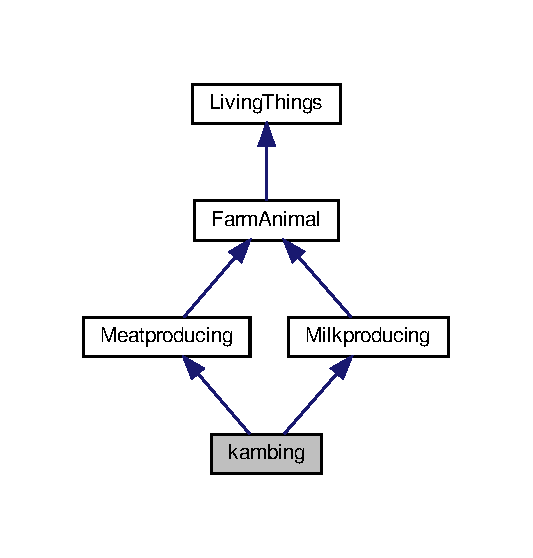
\includegraphics[width=256pt]{classkambing__inherit__graph}
\end{center}
\end{figure}


Collaboration diagram for kambing\+:
\nopagebreak
\begin{figure}[H]
\begin{center}
\leavevmode
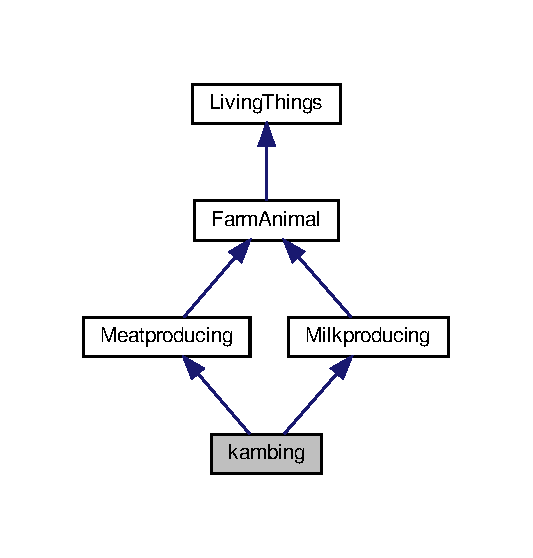
\includegraphics[width=256pt]{classkambing__coll__graph}
\end{center}
\end{figure}
\subsection*{Public Member Functions}
\begin{DoxyCompactItemize}
\item 
\mbox{\Hypertarget{classkambing_aada5f7194815a6ff15fef4fd12ddc2ce}\label{classkambing_aada5f7194815a6ff15fef4fd12ddc2ce}} 
{\bfseries kambing} (int posX, int posY)
\item 
\mbox{\Hypertarget{classkambing_af73a4db7712d8d97e8a0f48e2c6b47f0}\label{classkambing_af73a4db7712d8d97e8a0f48e2c6b47f0}} 
void {\bfseries move} ()
\item 
\mbox{\Hypertarget{classkambing_a9540126ad13162880929146d5a9ad473}\label{classkambing_a9540126ad13162880929146d5a9ad473}} 
void {\bfseries talk} ()
\item 
\mbox{\Hypertarget{classkambing_aca6072b89b48d7df2b3c34eecb31ca69}\label{classkambing_aca6072b89b48d7df2b3c34eecb31ca69}} 
void {\bfseries eat} ()
\item 
\mbox{\Hypertarget{classkambing_a9d043eee9316f7fefb0f15d16a50b116}\label{classkambing_a9d043eee9316f7fefb0f15d16a50b116}} 
string {\bfseries get\+Product} ()
\item 
\mbox{\Hypertarget{classkambing_a4e02d3e7e1684a14ad372e180adce2d2}\label{classkambing_a4e02d3e7e1684a14ad372e180adce2d2}} 
int {\bfseries getcountcow\+Milk} () const
\item 
\mbox{\Hypertarget{classkambing_a52c9800cebba7544eac66343261e192b}\label{classkambing_a52c9800cebba7544eac66343261e192b}} 
int {\bfseries get\+Full} ()
\item 
\mbox{\Hypertarget{classkambing_a2b3670a955dd6b7024eb2fa8dd4b0ed2}\label{classkambing_a2b3670a955dd6b7024eb2fa8dd4b0ed2}} 
void {\bfseries set\+Full} (int Full)
\end{DoxyCompactItemize}
\subsection*{Additional Inherited Members}


\subsection{Detailed Description}
kambing class. Classkambing ,turunan meat producing \begin{DoxyAuthor}{Author}
13517090 
\end{DoxyAuthor}
\begin{DoxySince}{Since}
2019.\+03.\+17 
\end{DoxySince}


The documentation for this class was generated from the following file\+:\begin{DoxyCompactItemize}
\item 
kambing.\+h\end{DoxyCompactItemize}

\hypertarget{classLambMeat}{}\section{Lamb\+Meat Class Reference}
\label{classLambMeat}\index{Lamb\+Meat@{Lamb\+Meat}}


{\ttfamily \#include $<$Lamb\+Meat.\+h$>$}



Inheritance diagram for Lamb\+Meat\+:
\nopagebreak
\begin{figure}[H]
\begin{center}
\leavevmode
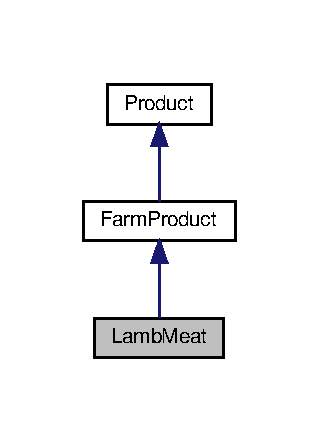
\includegraphics[width=153pt]{classLambMeat__inherit__graph}
\end{center}
\end{figure}


Collaboration diagram for Lamb\+Meat\+:
\nopagebreak
\begin{figure}[H]
\begin{center}
\leavevmode
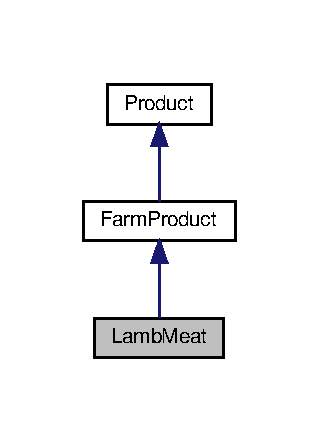
\includegraphics[width=153pt]{classLambMeat__coll__graph}
\end{center}
\end{figure}
\subsection*{Additional Inherited Members}


\subsection{Detailed Description}
\hyperlink{classLambMeat}{Lamb\+Meat} class.

\begin{DoxyAuthor}{Author}
Ghazwan S. M. \href{mailto:ghazwan.sihamudin@gmail.com}{\tt ghazwan.\+sihamudin@gmail.\+com} 
\end{DoxyAuthor}
\begin{DoxySince}{Since}
2019.\+03.\+17 
\end{DoxySince}


The documentation for this class was generated from the following files\+:\begin{DoxyCompactItemize}
\item 
Lamb\+Meat.\+h\item 
Lamb\+Meat.\+cpp\end{DoxyCompactItemize}

\hypertarget{classLand}{}\section{Land Class Reference}
\label{classLand}\index{Land@{Land}}


Inheritance diagram for Land\+:
\nopagebreak
\begin{figure}[H]
\begin{center}
\leavevmode
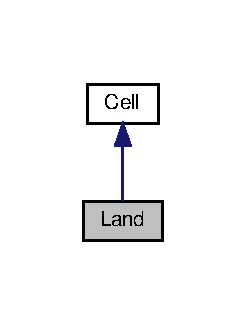
\includegraphics[width=118pt]{classLand__inherit__graph}
\end{center}
\end{figure}


Collaboration diagram for Land\+:
\nopagebreak
\begin{figure}[H]
\begin{center}
\leavevmode
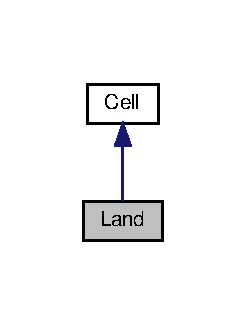
\includegraphics[width=118pt]{classLand__coll__graph}
\end{center}
\end{figure}
\subsection*{Public Member Functions}
\begin{DoxyCompactItemize}
\item 
\mbox{\Hypertarget{classLand_a3e3801a879d93123245ea44110bced34}\label{classLand_a3e3801a879d93123245ea44110bced34}} 
char {\bfseries get\+Element} (int x, int y)
\item 
\mbox{\Hypertarget{classLand_a777ba38407550c7868a6082913c56749}\label{classLand_a777ba38407550c7868a6082913c56749}} 
string {\bfseries get\+Properties} (char value)
\item 
\mbox{\Hypertarget{classLand_a9d172fde563a0e66ade4defaa70286db}\label{classLand_a9d172fde563a0e66ade4defaa70286db}} 
void {\bfseries set\+Element} (int x, int y, char e)
\end{DoxyCompactItemize}


The documentation for this class was generated from the following file\+:\begin{DoxyCompactItemize}
\item 
Land.\+h\end{DoxyCompactItemize}

\hypertarget{classLinkedList}{}\section{Linked\+List$<$ Type $>$ Class Template Reference}
\label{classLinkedList}\index{Linked\+List$<$ Type $>$@{Linked\+List$<$ Type $>$}}
\subsection*{Public Member Functions}
\begin{DoxyCompactItemize}
\item 
\mbox{\Hypertarget{classLinkedList_a28583dab40155730c7e83270b911317d}\label{classLinkedList_a28583dab40155730c7e83270b911317d}} 
int {\bfseries find} (Type element)
\item 
\mbox{\Hypertarget{classLinkedList_a1164e950c11d424cc8a50f7419b3990e}\label{classLinkedList_a1164e950c11d424cc8a50f7419b3990e}} 
bool {\bfseries is\+Empty} ()
\item 
\mbox{\Hypertarget{classLinkedList_aa138117192ac2a5bdb056092bcd1cd25}\label{classLinkedList_aa138117192ac2a5bdb056092bcd1cd25}} 
void {\bfseries add} (Type element)
\item 
\mbox{\Hypertarget{classLinkedList_a16c240dca90856ca78c51c61d7d5e7e1}\label{classLinkedList_a16c240dca90856ca78c51c61d7d5e7e1}} 
void {\bfseries remove} (Type element)
\item 
\mbox{\Hypertarget{classLinkedList_a0362da1e1041e749c3d75dc3628186e9}\label{classLinkedList_a0362da1e1041e749c3d75dc3628186e9}} 
Type {\bfseries get} (int indeks)
\item 
\mbox{\Hypertarget{classLinkedList_a2da81f9d412159a0d1a1c9e2ed3112a1}\label{classLinkedList_a2da81f9d412159a0d1a1c9e2ed3112a1}} 
int {\bfseries get\+Size} ()
\item 
\mbox{\Hypertarget{classLinkedList_af8475b3b2da84ebd7c3af2358df825d2}\label{classLinkedList_af8475b3b2da84ebd7c3af2358df825d2}} 
void {\bfseries print} ()
\end{DoxyCompactItemize}


The documentation for this class was generated from the following files\+:\begin{DoxyCompactItemize}
\item 
Linked\+List.\+h\item 
Linked\+List.\+cpp\end{DoxyCompactItemize}

\hypertarget{classLivingThings}{}\section{Living\+Things Class Reference}
\label{classLivingThings}\index{Living\+Things@{Living\+Things}}


Inheritance diagram for Living\+Things\+:
\nopagebreak
\begin{figure}[H]
\begin{center}
\leavevmode
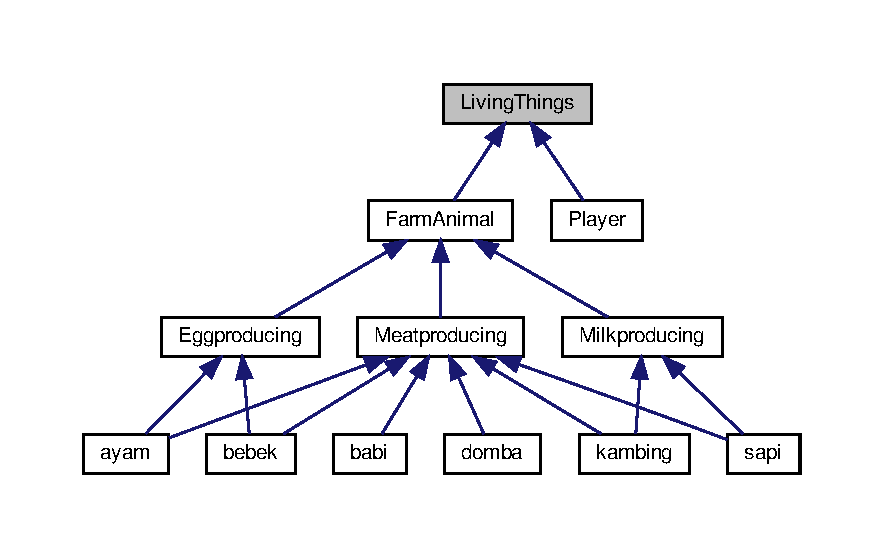
\includegraphics[width=350pt]{classLivingThings__inherit__graph}
\end{center}
\end{figure}
\subsection*{Public Member Functions}
\begin{DoxyCompactItemize}
\item 
\mbox{\Hypertarget{classLivingThings_a2277af0cf3a294a7e17f2a6e01ba0d84}\label{classLivingThings_a2277af0cf3a294a7e17f2a6e01ba0d84}} 
virtual void {\bfseries talk} ()=0
\end{DoxyCompactItemize}


The documentation for this class was generated from the following file\+:\begin{DoxyCompactItemize}
\item 
Living\+Things.\+h\end{DoxyCompactItemize}

\hypertarget{classMeatproducing}{}\section{Meatproducing Class Reference}
\label{classMeatproducing}\index{Meatproducing@{Meatproducing}}


{\ttfamily \#include $<$Meatproducing.\+h$>$}



Inheritance diagram for Meatproducing\+:
\nopagebreak
\begin{figure}[H]
\begin{center}
\leavevmode
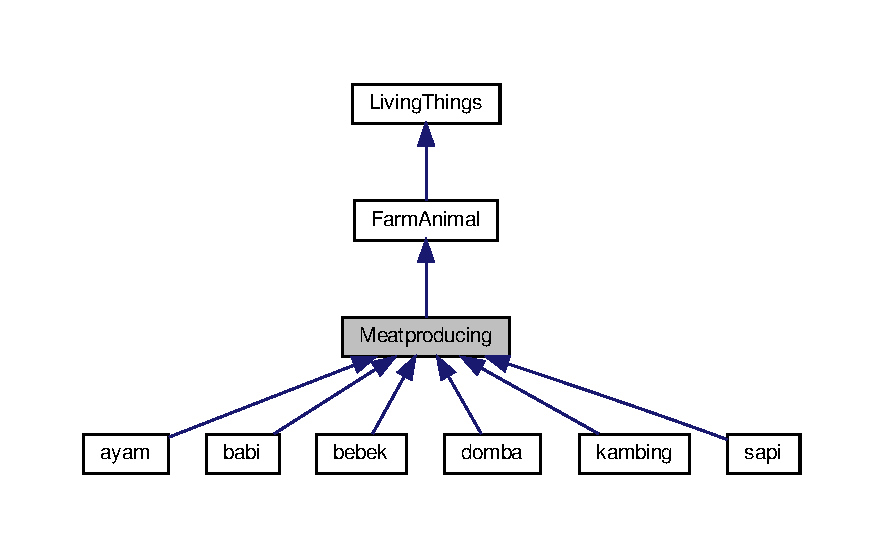
\includegraphics[width=350pt]{classMeatproducing__inherit__graph}
\end{center}
\end{figure}


Collaboration diagram for Meatproducing\+:
\nopagebreak
\begin{figure}[H]
\begin{center}
\leavevmode
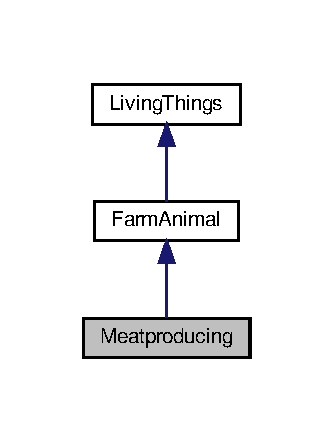
\includegraphics[width=160pt]{classMeatproducing__coll__graph}
\end{center}
\end{figure}
\subsection*{Public Member Functions}
\begin{DoxyCompactItemize}
\item 
\mbox{\Hypertarget{classMeatproducing_a5f7d6e507dd62044029052e805cd37dd}\label{classMeatproducing_a5f7d6e507dd62044029052e805cd37dd}} 
{\bfseries Meatproducing} (int x, int y)
\end{DoxyCompactItemize}
\subsection*{Static Public Member Functions}
\begin{DoxyCompactItemize}
\item 
\mbox{\Hypertarget{classMeatproducing_ad3370dd411d1a8c60ad0a8ee42c9308e}\label{classMeatproducing_ad3370dd411d1a8c60ad0a8ee42c9308e}} 
static int {\bfseries getjlh\+MeatP} ()
\end{DoxyCompactItemize}
\subsection*{Additional Inherited Members}


\subsection{Detailed Description}
\hyperlink{classMeatproducing}{Meatproducing} class Class hewan penghasil daging,kelas turunan dari farm animal \begin{DoxyAuthor}{Author}
13517090 
\end{DoxyAuthor}
\begin{DoxySince}{Since}
2019.\+03.\+17 
\end{DoxySince}


The documentation for this class was generated from the following file\+:\begin{DoxyCompactItemize}
\item 
Meatproducing.\+h\end{DoxyCompactItemize}

\hypertarget{classMilkproducing}{}\section{Milkproducing Class Reference}
\label{classMilkproducing}\index{Milkproducing@{Milkproducing}}


Inheritance diagram for Milkproducing\+:
\nopagebreak
\begin{figure}[H]
\begin{center}
\leavevmode
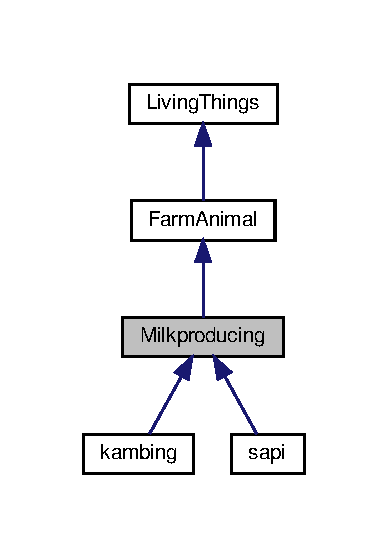
\includegraphics[width=186pt]{classMilkproducing__inherit__graph}
\end{center}
\end{figure}


Collaboration diagram for Milkproducing\+:
\nopagebreak
\begin{figure}[H]
\begin{center}
\leavevmode
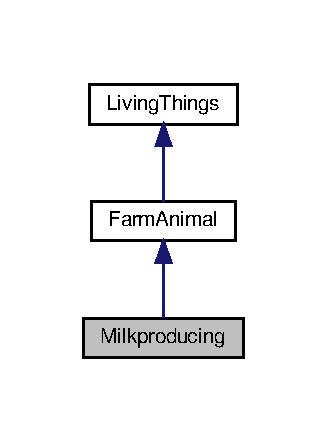
\includegraphics[width=157pt]{classMilkproducing__coll__graph}
\end{center}
\end{figure}
\subsection*{Public Member Functions}
\begin{DoxyCompactItemize}
\item 
\mbox{\Hypertarget{classMilkproducing_a74aa25fa5febb55d3e422cebd2d6687a}\label{classMilkproducing_a74aa25fa5febb55d3e422cebd2d6687a}} 
{\bfseries Milkproducing} (int x, int y)
\end{DoxyCompactItemize}
\subsection*{Static Public Member Functions}
\begin{DoxyCompactItemize}
\item 
\mbox{\Hypertarget{classMilkproducing_a7ee5abf21d8711db0aa5b4060318aa95}\label{classMilkproducing_a7ee5abf21d8711db0aa5b4060318aa95}} 
static int {\bfseries getjlh\+MilkP} ()
\end{DoxyCompactItemize}
\subsection*{Additional Inherited Members}


The documentation for this class was generated from the following files\+:\begin{DoxyCompactItemize}
\item 
Milkproducing.\+h\item 
Milkproducing.\+cpp\end{DoxyCompactItemize}

\hypertarget{structnode}{}\section{node$<$ Type $>$ Struct Template Reference}
\label{structnode}\index{node$<$ Type $>$@{node$<$ Type $>$}}
\subsection*{Public Attributes}
\begin{DoxyCompactItemize}
\item 
\mbox{\Hypertarget{structnode_a89b6482e263bd001b885949460b85766}\label{structnode_a89b6482e263bd001b885949460b85766}} 
\hyperlink{structnode}{node}$<$ Type $>$ $\ast$ {\bfseries next}
\item 
\mbox{\Hypertarget{structnode_a83df696cde0652190a47af4c03b52f5e}\label{structnode_a83df696cde0652190a47af4c03b52f5e}} 
Type {\bfseries data}
\end{DoxyCompactItemize}


The documentation for this struct was generated from the following file\+:\begin{DoxyCompactItemize}
\item 
Linked\+List.\+h\end{DoxyCompactItemize}

\hypertarget{classOmelette}{}\section{Omelette Class Reference}
\label{classOmelette}\index{Omelette@{Omelette}}


{\ttfamily \#include $<$Omelette.\+h$>$}



Inheritance diagram for Omelette\+:
\nopagebreak
\begin{figure}[H]
\begin{center}
\leavevmode
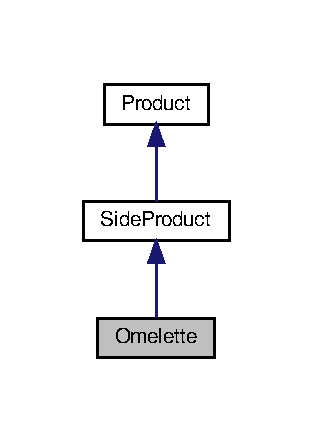
\includegraphics[width=150pt]{classOmelette__inherit__graph}
\end{center}
\end{figure}


Collaboration diagram for Omelette\+:
\nopagebreak
\begin{figure}[H]
\begin{center}
\leavevmode
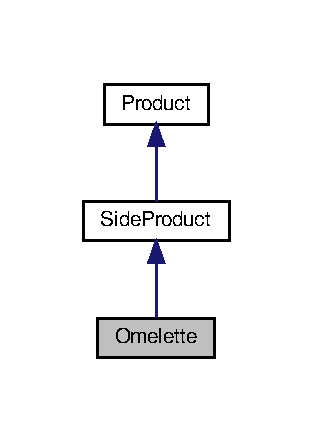
\includegraphics[width=150pt]{classOmelette__coll__graph}
\end{center}
\end{figure}
\subsection*{Public Member Functions}
\begin{DoxyCompactItemize}
\item 
\mbox{\Hypertarget{classOmelette_a9de6bf62fb9cfad149092418704da6d2}\label{classOmelette_a9de6bf62fb9cfad149092418704da6d2}} 
{\bfseries Omelette} (int portion)
\end{DoxyCompactItemize}
\subsection*{Additional Inherited Members}


\subsection{Detailed Description}
\hyperlink{classOmelette}{Omelette} class.

\begin{DoxyAuthor}{Author}
Ghazwan S. M. \href{mailto:ghazwan.sihamudin@gmail.com}{\tt ghazwan.\+sihamudin@gmail.\+com} 
\end{DoxyAuthor}
\begin{DoxySince}{Since}
2019.\+03.\+17 
\end{DoxySince}


The documentation for this class was generated from the following files\+:\begin{DoxyCompactItemize}
\item 
Omelette.\+h\item 
Omelette.\+cpp\end{DoxyCompactItemize}

\hypertarget{classPlayer}{}\section{Player Class Reference}
\label{classPlayer}\index{Player@{Player}}


Inheritance diagram for Player\+:
\nopagebreak
\begin{figure}[H]
\begin{center}
\leavevmode
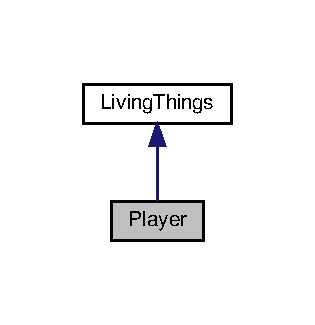
\includegraphics[width=148pt]{classPlayer__inherit__graph}
\end{center}
\end{figure}


Collaboration diagram for Player\+:
\nopagebreak
\begin{figure}[H]
\begin{center}
\leavevmode
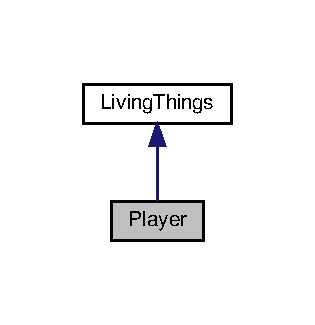
\includegraphics[width=148pt]{classPlayer__coll__graph}
\end{center}
\end{figure}
\subsection*{Public Member Functions}
\begin{DoxyCompactItemize}
\item 
\mbox{\Hypertarget{classPlayer_a9b009cc0bebdcc27a837d50b1f4ededd}\label{classPlayer_a9b009cc0bebdcc27a837d50b1f4ededd}} 
{\bfseries Player} (int x, int y)
\item 
\mbox{\Hypertarget{classPlayer_a7397d7b5cde969d16d42fadfbbdf5ed6}\label{classPlayer_a7397d7b5cde969d16d42fadfbbdf5ed6}} 
Hanya dapat bergerak petak per {\bfseries pemanggilan} (?) ato enggak $\ast$/void Move(int posX
\item 
\mbox{\Hypertarget{classPlayer_aea0a70d3ccb250dffab89aadcf24da7d}\label{classPlayer_aea0a70d3ccb250dffab89aadcf24da7d}} 
void {\bfseries Talk} ()
\item 
\mbox{\Hypertarget{classPlayer_a8e37426c9e431828f67840b507b0d2ef}\label{classPlayer_a8e37426c9e431828f67840b507b0d2ef}} 
void {\bfseries Interact} ()
\item 
\mbox{\Hypertarget{classPlayer_a0c74d6bd430490417bb34e9abc233bb7}\label{classPlayer_a0c74d6bd430490417bb34e9abc233bb7}} 
void {\bfseries Kill} ()
\item 
\mbox{\Hypertarget{classPlayer_a91c92058dc2edc2a2a954abb6806cf3a}\label{classPlayer_a91c92058dc2edc2a2a954abb6806cf3a}} 
void {\bfseries Grow} ()
\end{DoxyCompactItemize}
\subsection*{Public Attributes}
\begin{DoxyCompactItemize}
\item 
\mbox{\Hypertarget{classPlayer_a877e264962066a3d85e6a3bd5ea4a161}\label{classPlayer_a877e264962066a3d85e6a3bd5ea4a161}} 
Hanya dapat bergerak petak per int {\bfseries posY}
\end{DoxyCompactItemize}


The documentation for this class was generated from the following file\+:\begin{DoxyCompactItemize}
\item 
Player.\+h\end{DoxyCompactItemize}

\hypertarget{classPork}{}\section{Pork Class Reference}
\label{classPork}\index{Pork@{Pork}}


{\ttfamily \#include $<$Pork.\+h$>$}



Inheritance diagram for Pork\+:
\nopagebreak
\begin{figure}[H]
\begin{center}
\leavevmode
\includegraphics[width=153pt]{classPork__inherit__graph}
\end{center}
\end{figure}


Collaboration diagram for Pork\+:
\nopagebreak
\begin{figure}[H]
\begin{center}
\leavevmode
\includegraphics[width=153pt]{classPork__coll__graph}
\end{center}
\end{figure}
\subsection*{Additional Inherited Members}


\subsection{Detailed Description}
\hyperlink{classPork}{Pork} class.

\begin{DoxyAuthor}{Author}
Ghazwan S. M. \href{mailto:ghazwan.sihamudin@gmail.com}{\tt ghazwan.\+sihamudin@gmail.\+com} 
\end{DoxyAuthor}
\begin{DoxySince}{Since}
2019.\+03.\+17 
\end{DoxySince}


The documentation for this class was generated from the following files\+:\begin{DoxyCompactItemize}
\item 
Pork.\+h\item 
Pork.\+cpp\end{DoxyCompactItemize}

\hypertarget{classProduct}{}\section{Product Class Reference}
\label{classProduct}\index{Product@{Product}}


{\ttfamily \#include $<$Product.\+h$>$}



Inheritance diagram for Product\+:
\nopagebreak
\begin{figure}[H]
\begin{center}
\leavevmode
\includegraphics[width=349pt]{classProduct__inherit__graph}
\end{center}
\end{figure}
\subsection*{Public Member Functions}
\begin{DoxyCompactItemize}
\item 
int \hyperlink{classProduct_a3d0f4dafb8cfe6a3d90fd661dc6cb2d0}{get\+Product\+Value} ()
\item 
int \hyperlink{classProduct_af1bdfcee872537bb8492160109aa7fb3}{get\+Expire\+Value} ()
\end{DoxyCompactItemize}
\subsection*{Public Attributes}
\begin{DoxyCompactItemize}
\item 
\mbox{\Hypertarget{classProduct_af9e601cc45c4281a39e7f4cbdf4d2a53}\label{classProduct_af9e601cc45c4281a39e7f4cbdf4d2a53}} 
int {\bfseries expire\+Value}
\end{DoxyCompactItemize}


\subsection{Detailed Description}
\hyperlink{classProduct}{Product} class.

\begin{DoxyAuthor}{Author}
Ghazwan S. M. \href{mailto:ghazwan.sihamudin@gmail.com}{\tt ghazwan.\+sihamudin@gmail.\+com} 
\end{DoxyAuthor}
\begin{DoxySince}{Since}
2019.\+03.\+17 
\end{DoxySince}


\subsection{Member Function Documentation}
\mbox{\Hypertarget{classProduct_af1bdfcee872537bb8492160109aa7fb3}\label{classProduct_af1bdfcee872537bb8492160109aa7fb3}} 
\index{Product@{Product}!get\+Expire\+Value@{get\+Expire\+Value}}
\index{get\+Expire\+Value@{get\+Expire\+Value}!Product@{Product}}
\subsubsection{\texorpdfstring{get\+Expire\+Value()}{getExpireValue()}}
{\footnotesize\ttfamily int Product\+::get\+Expire\+Value (\begin{DoxyParamCaption}{ }\end{DoxyParamCaption})}

Get the expire value of the product. \begin{DoxyReturn}{Returns}
int expire value. 
\end{DoxyReturn}
\mbox{\Hypertarget{classProduct_a3d0f4dafb8cfe6a3d90fd661dc6cb2d0}\label{classProduct_a3d0f4dafb8cfe6a3d90fd661dc6cb2d0}} 
\index{Product@{Product}!get\+Product\+Value@{get\+Product\+Value}}
\index{get\+Product\+Value@{get\+Product\+Value}!Product@{Product}}
\subsubsection{\texorpdfstring{get\+Product\+Value()}{getProductValue()}}
{\footnotesize\ttfamily int Product\+::get\+Product\+Value (\begin{DoxyParamCaption}{ }\end{DoxyParamCaption})}

Get the product value. \begin{DoxyReturn}{Returns}
int product value. 
\end{DoxyReturn}


The documentation for this class was generated from the following file\+:\begin{DoxyCompactItemize}
\item 
Product.\+h\end{DoxyCompactItemize}

\hypertarget{classRenderable}{}\section{Renderable Class Reference}
\label{classRenderable}\index{Renderable@{Renderable}}
\subsection*{Public Member Functions}
\begin{DoxyCompactItemize}
\item 
\mbox{\Hypertarget{classRenderable_a7d02709d871bd2bde97d41d933df5adf}\label{classRenderable_a7d02709d871bd2bde97d41d933df5adf}} 
virtual void {\bfseries render} ()=0
\end{DoxyCompactItemize}


The documentation for this class was generated from the following file\+:\begin{DoxyCompactItemize}
\item 
Renderable.\+h\end{DoxyCompactItemize}

\hypertarget{classsapi}{}\section{sapi Class Reference}
\label{classsapi}\index{sapi@{sapi}}


Inheritance diagram for sapi\+:
\nopagebreak
\begin{figure}[H]
\begin{center}
\leavevmode
\includegraphics[width=256pt]{classsapi__inherit__graph}
\end{center}
\end{figure}


Collaboration diagram for sapi\+:
\nopagebreak
\begin{figure}[H]
\begin{center}
\leavevmode
\includegraphics[width=256pt]{classsapi__coll__graph}
\end{center}
\end{figure}
\subsection*{Public Member Functions}
\begin{DoxyCompactItemize}
\item 
\mbox{\Hypertarget{classsapi_a62abc4f374396934025399c7717c6403}\label{classsapi_a62abc4f374396934025399c7717c6403}} 
{\bfseries sapi} (int posX, int posY)
\item 
\mbox{\Hypertarget{classsapi_a624bca7575e1fdecdcc8ac38ab662a9a}\label{classsapi_a624bca7575e1fdecdcc8ac38ab662a9a}} 
void {\bfseries move} (\hyperlink{classCell}{Cell} \&\+\_\+c)
\item 
\mbox{\Hypertarget{classsapi_a394f5198322bce5ddff6073207112021}\label{classsapi_a394f5198322bce5ddff6073207112021}} 
void {\bfseries talk} ()
\item 
\mbox{\Hypertarget{classsapi_a6bb4f1e7efd67963063c96ffe741d34c}\label{classsapi_a6bb4f1e7efd67963063c96ffe741d34c}} 
void {\bfseries eat} (\hyperlink{classCell}{Cell} \&\+\_\+c)
\item 
\mbox{\Hypertarget{classsapi_a63b013c6a91f03241f3d59fda2ec4376}\label{classsapi_a63b013c6a91f03241f3d59fda2ec4376}} 
string {\bfseries get\+Char} ()
\item 
\mbox{\Hypertarget{classsapi_aa300fe6b4b07e094cb712cd176fa94ee}\label{classsapi_aa300fe6b4b07e094cb712cd176fa94ee}} 
void {\bfseries get\+Product} ()
\item 
\mbox{\Hypertarget{classsapi_ab8c576b92810a66d735dc40fa2d33430}\label{classsapi_ab8c576b92810a66d735dc40fa2d33430}} 
int {\bfseries get\+Count\+Cow\+Milk} () const
\item 
\mbox{\Hypertarget{classsapi_ac2cea89f18795443a7ddb87d871768a0}\label{classsapi_ac2cea89f18795443a7ddb87d871768a0}} 
int {\bfseries get\+Full} ()
\item 
\mbox{\Hypertarget{classsapi_a24a69158e59a6b8fab669517626e7d03}\label{classsapi_a24a69158e59a6b8fab669517626e7d03}} 
void {\bfseries set\+Full} (int Full)
\item 
\mbox{\Hypertarget{classsapi_ad39e03499c3e5870ab68fd9594ddae11}\label{classsapi_ad39e03499c3e5870ab68fd9594ddae11}} 
void {\bfseries Print} ()
\end{DoxyCompactItemize}
\subsection*{Additional Inherited Members}


The documentation for this class was generated from the following files\+:\begin{DoxyCompactItemize}
\item 
sapi.\+h\item 
sapi.\+cpp\end{DoxyCompactItemize}

\hypertarget{classSausage}{}\section{Sausage Class Reference}
\label{classSausage}\index{Sausage@{Sausage}}


{\ttfamily \#include $<$Sausage.\+h$>$}



Inheritance diagram for Sausage\+:
\nopagebreak
\begin{figure}[H]
\begin{center}
\leavevmode
\includegraphics[width=150pt]{classSausage__inherit__graph}
\end{center}
\end{figure}


Collaboration diagram for Sausage\+:
\nopagebreak
\begin{figure}[H]
\begin{center}
\leavevmode
\includegraphics[width=150pt]{classSausage__coll__graph}
\end{center}
\end{figure}
\subsection*{Public Member Functions}
\begin{DoxyCompactItemize}
\item 
\mbox{\Hypertarget{classSausage_a04febb9bb976bb9054aac77465b5186b}\label{classSausage_a04febb9bb976bb9054aac77465b5186b}} 
{\bfseries Sausage} (int portion)
\end{DoxyCompactItemize}
\subsection*{Additional Inherited Members}


\subsection{Detailed Description}
\hyperlink{classSausage}{Sausage} class.

\begin{DoxyAuthor}{Author}
Ghazwan S. M. \href{mailto:ghazwan.sihamudin@gmail.com}{\tt ghazwan.\+sihamudin@gmail.\+com} 
\end{DoxyAuthor}
\begin{DoxySince}{Since}
2019.\+03.\+17 
\end{DoxySince}


The documentation for this class was generated from the following files\+:\begin{DoxyCompactItemize}
\item 
Sausage.\+h\item 
Sausage.\+cpp\end{DoxyCompactItemize}

\hypertarget{classSideProduct}{}\section{Side\+Product Class Reference}
\label{classSideProduct}\index{Side\+Product@{Side\+Product}}


{\ttfamily \#include $<$Side\+Product.\+h$>$}



Inheritance diagram for Side\+Product\+:
\nopagebreak
\begin{figure}[H]
\begin{center}
\leavevmode
\includegraphics[width=266pt]{classSideProduct__inherit__graph}
\end{center}
\end{figure}


Collaboration diagram for Side\+Product\+:
\nopagebreak
\begin{figure}[H]
\begin{center}
\leavevmode
\includegraphics[width=150pt]{classSideProduct__coll__graph}
\end{center}
\end{figure}
\subsection*{Public Member Functions}
\begin{DoxyCompactItemize}
\item 
int \hyperlink{classSideProduct_a8265dbcfcde3880817bfb8d82e563700}{get\+Portion} ()
\item 
int \hyperlink{classSideProduct_ae37e75482c8ddaf7abe070054fad58eb}{get\+Product\+Value} ()
\item 
int \hyperlink{classSideProduct_a2ea1a135e6456d0220f3ba3d3e8c9dfb}{get\+Expire\+Value} ()
\item 
void \hyperlink{classSideProduct_abff90c90ea13a3511dcd8dbdf55fc33c}{set\+Expire\+Value} ()
\item 
bool \hyperlink{classSideProduct_a9a37b515860c516ec28749f5b562aa0f}{is\+Expire} ()
\end{DoxyCompactItemize}
\subsection*{Protected Attributes}
\begin{DoxyCompactItemize}
\item 
\mbox{\Hypertarget{classSideProduct_a92b465582932a080a9080e9bc748f104}\label{classSideProduct_a92b465582932a080a9080e9bc748f104}} 
int {\bfseries portion}
\end{DoxyCompactItemize}


\subsection{Detailed Description}
\hyperlink{classSideProduct}{Side\+Product} class.

\begin{DoxyAuthor}{Author}
Ghazwan S. M. \href{mailto:ghazwan.sihamudin@gmail.com}{\tt ghazwan.\+sihamudin@gmail.\+com} 
\end{DoxyAuthor}
\begin{DoxySince}{Since}
2019.\+03.\+17 
\end{DoxySince}


\subsection{Member Function Documentation}
\mbox{\Hypertarget{classSideProduct_a2ea1a135e6456d0220f3ba3d3e8c9dfb}\label{classSideProduct_a2ea1a135e6456d0220f3ba3d3e8c9dfb}} 
\index{Side\+Product@{Side\+Product}!get\+Expire\+Value@{get\+Expire\+Value}}
\index{get\+Expire\+Value@{get\+Expire\+Value}!Side\+Product@{Side\+Product}}
\subsubsection{\texorpdfstring{get\+Expire\+Value()}{getExpireValue()}}
{\footnotesize\ttfamily int Side\+Product\+::get\+Expire\+Value (\begin{DoxyParamCaption}{ }\end{DoxyParamCaption})\hspace{0.3cm}{\ttfamily [virtual]}}

Get the expire value of the product. \begin{DoxyReturn}{Returns}
int expire value. 
\end{DoxyReturn}


Implements \hyperlink{classProduct_a739031c520fb9e376da3d3fc2955c7e7}{Product}.

\mbox{\Hypertarget{classSideProduct_a8265dbcfcde3880817bfb8d82e563700}\label{classSideProduct_a8265dbcfcde3880817bfb8d82e563700}} 
\index{Side\+Product@{Side\+Product}!get\+Portion@{get\+Portion}}
\index{get\+Portion@{get\+Portion}!Side\+Product@{Side\+Product}}
\subsubsection{\texorpdfstring{get\+Portion()}{getPortion()}}
{\footnotesize\ttfamily int Side\+Product\+::get\+Portion (\begin{DoxyParamCaption}{ }\end{DoxyParamCaption})}

Get product portion. \begin{DoxyReturn}{Returns}
int portion. 
\end{DoxyReturn}
\mbox{\Hypertarget{classSideProduct_ae37e75482c8ddaf7abe070054fad58eb}\label{classSideProduct_ae37e75482c8ddaf7abe070054fad58eb}} 
\index{Side\+Product@{Side\+Product}!get\+Product\+Value@{get\+Product\+Value}}
\index{get\+Product\+Value@{get\+Product\+Value}!Side\+Product@{Side\+Product}}
\subsubsection{\texorpdfstring{get\+Product\+Value()}{getProductValue()}}
{\footnotesize\ttfamily int Side\+Product\+::get\+Product\+Value (\begin{DoxyParamCaption}{ }\end{DoxyParamCaption})\hspace{0.3cm}{\ttfamily [virtual]}}

Get the product value. \begin{DoxyReturn}{Returns}
int product value. 
\end{DoxyReturn}


Implements \hyperlink{classProduct_a5c56d625cae28f43b626578ac4611e43}{Product}.

\mbox{\Hypertarget{classSideProduct_a9a37b515860c516ec28749f5b562aa0f}\label{classSideProduct_a9a37b515860c516ec28749f5b562aa0f}} 
\index{Side\+Product@{Side\+Product}!is\+Expire@{is\+Expire}}
\index{is\+Expire@{is\+Expire}!Side\+Product@{Side\+Product}}
\subsubsection{\texorpdfstring{is\+Expire()}{isExpire()}}
{\footnotesize\ttfamily bool Side\+Product\+::is\+Expire (\begin{DoxyParamCaption}{ }\end{DoxyParamCaption})\hspace{0.3cm}{\ttfamily [virtual]}}

Get the product expire condition. \begin{DoxyReturn}{Returns}
bool expire condition. 
\end{DoxyReturn}


Implements \hyperlink{classProduct_aec86d25d77417014f8780ea65416bac7}{Product}.

\mbox{\Hypertarget{classSideProduct_abff90c90ea13a3511dcd8dbdf55fc33c}\label{classSideProduct_abff90c90ea13a3511dcd8dbdf55fc33c}} 
\index{Side\+Product@{Side\+Product}!set\+Expire\+Value@{set\+Expire\+Value}}
\index{set\+Expire\+Value@{set\+Expire\+Value}!Side\+Product@{Side\+Product}}
\subsubsection{\texorpdfstring{set\+Expire\+Value()}{setExpireValue()}}
{\footnotesize\ttfamily void Side\+Product\+::set\+Expire\+Value (\begin{DoxyParamCaption}{ }\end{DoxyParamCaption})\hspace{0.3cm}{\ttfamily [virtual]}}

Reduce the expire value of the product by 1. 

Implements \hyperlink{classProduct_a84aba139efc9cbcb05d47de168645463}{Product}.



The documentation for this class was generated from the following files\+:\begin{DoxyCompactItemize}
\item 
Side\+Product.\+h\item 
Side\+Product.\+cpp\end{DoxyCompactItemize}

%--- End generated contents ---

% Index
\backmatter
\newpage
\phantomsection
\clearemptydoublepage
\addcontentsline{toc}{chapter}{Index}
\printindex

\end{document}
